% =============================================================================
%  NEJM AI — Original Article Manuscript & Supplementary Appendix
%  Hospital-Disjoint and In-Network Pre-Incision POAF Prediction (STS ACSD v2.81)
%  Format: NEJM Group editorial styling — Bitstream Charter serif body,
%          clean sans-serif display headings, NEJM Crimson (#9E1B32) & Navy
%          (#1B365D) palette, structured 250-word abstract, IMRaD body,
%          superscript sequential Vancouver references, TRIPOD+AI Supplement.
% =============================================================================
\documentclass[10pt,letterpaper,twocolumn]{article}
\pdfminorversion=7

% ---- fonts & microtypography -------------------------------------------------
\usepackage[T1]{fontenc}
\usepackage[utf8]{inputenc}
\usepackage{amsmath,amssymb}
\usepackage{txfonts}
\usepackage{charter}
\usepackage[scaled=0.88]{helvet}
\renewcommand{\ttdefault}{lmtt}
\usepackage[italic,defaultmathsizes]{mathastext}
\makeatletter
\DeclareSymbolFontAlphabet{\mathrm}{mtoperatorfont}
\renewcommand{\operator@font}{\mathgroup\symmtoperatorfont}
\makeatother
\usepackage[protrusion=true,expansion=true,final]{microtype}
\DisableLigatures[-]{encoding = T1, family = tt*}

% ---- geometry ----------------------------------------------------------------
\usepackage[letterpaper,left=0.72in,right=0.72in,top=0.88in,bottom=0.85in,
            columnsep=0.27in,headheight=19pt,headsep=0.22in,footskip=0.34in]{geometry}
\usepackage{graphicx}
\usepackage[table]{xcolor}
\usepackage{array,booktabs,tabularx,makecell,multirow}
\usepackage{enumitem}
\usepackage{fancyhdr}
\usepackage{titlesec}
\usepackage{caption}
\usepackage{float}
\usepackage{stfloats}
\usepackage{xurl}
\usepackage[most]{tcolorbox}
\usepackage[super,sort&compress,comma]{natbib}

% ---- NEJM AI Editorial Palette -----------------------------------------------
\definecolor{ink}{HTML}{111827}
\definecolor{sub}{HTML}{374151}
\definecolor{muted}{HTML}{6B7280}
\definecolor{hair}{HTML}{D1D5DB}
\definecolor{surface}{HTML}{F7F8FA}
\definecolor{crimson}{HTML}{9E1B32}
\definecolor{crimsondark}{HTML}{7A1224}
\definecolor{primarytint}{HTML}{FBF0F2}
\definecolor{navy}{HTML}{1B365D}
\definecolor{teal}{HTML}{0F6E6E}
\definecolor{blue}{HTML}{2B5B84}

% ---- hyperlinks & PDF metadata -----------------------------------------------
\newcommand{\papertitle}{Continuous-Target Learning and Parallel Genetic Programming for Pre-Incision Postoperative Atrial Fibrillation Prediction Across Unseen and Seen U.S.\ Hospitals}
\newcommand{\shorttitle}{Pre-Incision POAF Prediction Across 1,091 U.S.\ Hospitals}
\usepackage[colorlinks=true,linkcolor=crimson,citecolor=navy,urlcolor=blue,
            bookmarksnumbered=true]{hyperref}
\hypersetup{
  pdftitle={\papertitle},
  pdfauthor={Jepson Taylor, Zain Khalpey, Ricky Ray Butler, Jordan Morrow, Alton Alexander, Jordan Hildebrandt, Besterlyne Jirongo},
  pdfsubject={NEJM AI Original Article — National STS ACSD v2.81 Isolated-CABG POAF Benchmark},
  pdfkeywords={postoperative atrial fibrillation, STS ACSD, CABG, NEJM AI, hospital-disjoint validation, seen-hospital calibration, tabular foundation models, EvoTarget-FT, JAIN Ultra GP v2}
}
\urlstyle{same}

% ---- rhythm & float control --------------------------------------------------
\linespread{1.04}
\setlength{\parindent}{1.05em}
\setlength{\parskip}{0pt}
\emergencystretch=1.2em
\raggedbottom
\clubpenalty=6000 \widowpenalty=6000
\setlist{leftmargin=1.45em,itemsep=2pt,topsep=3.5pt,parsep=0pt}
\renewcommand{\topfraction}{0.92}
\renewcommand{\dbltopfraction}{0.92}
\renewcommand{\bottomfraction}{0.60}
\renewcommand{\textfraction}{0.06}
\renewcommand{\floatpagefraction}{0.85}
\renewcommand{\dblfloatpagefraction}{0.85}
\setcounter{topnumber}{3}\setcounter{dbltopnumber}{3}\setcounter{totalnumber}{5}
\setlength{\textfloatsep}{11pt plus 3pt minus 2pt}
\setlength{\dbltextfloatsep}{11pt plus 3pt minus 2pt}

% ---- NEJM Editorial Headings -------------------------------------------------
\titleformat{\section}{\sffamily\bfseries\fontsize{10.5}{12.5}\selectfont\color{crimson}}
  {}{0pt}{\MakeUppercase}[\vspace{2pt}{\color{hair}\titlerule[0.5pt]}]
\titlespacing*{\section}{0pt}{13pt plus 3pt minus 2pt}{5pt plus 1pt}
\titleformat{\subsection}{\sffamily\bfseries\fontsize{9.2}{11.2}\selectfont\color{navy}\raggedright}
  {}{0pt}{}
\titlespacing*{\subsection}{0pt}{8.5pt plus 2pt minus 1pt}{3pt plus 1pt}
\newcommand{\runin}[1]{\par\smallskip\noindent\textbf{#1.}\hspace{0.4em}\ignorespaces}

% ---- running headers & footers -----------------------------------------------
\pagestyle{fancy}\fancyhf{}
\renewcommand{\headrulewidth}{0.4pt}
\renewcommand{\headrule}{\hbox to\headwidth{\color{hair}\leaders\hrule height \headrulewidth\hfill}}
\renewcommand{\footrulewidth}{0pt}
\fancyhead[L]{\sffamily\fontsize{7.4}{9}\selectfont\textcolor{crimson}{\textbf{NEJM AI}}\hspace{0.7em}\textcolor{muted}{|}\hspace{0.7em}\textcolor{sub}{\shorttitle}}
\fancyhead[R]{\sffamily\fontsize{7.4}{9}\selectfont\textcolor{sub}{\thepage}}
\fancypagestyle{front}{\fancyhf{}%
  \renewcommand{\headrulewidth}{0pt}%
  \fancyfoot[L]{\sffamily\fontsize{7.3}{9}\selectfont\textcolor{muted}{Original Article Submission Manuscript — Prepared in NEJM AI Editorial Format}}%
  \fancyfoot[R]{\sffamily\fontsize{7.3}{9}\selectfont\textcolor{sub}{\thepage}}}

% ---- captions ----------------------------------------------------------------
\DeclareCaptionLabelFormat{nejm}{\textcolor{crimson}{\bfseries #1~#2.}}
\DeclareCaptionLabelSeparator{nejmsep}{\hspace{0.45em}}
\DeclareCaptionFont{nejmfont}{\sffamily\fontsize{7.8}{10.0}\selectfont\color{sub}}
\captionsetup{font=nejmfont,labelformat=nejm,labelsep=nejmsep,
              justification=raggedright,singlelinecheck=false,skip=5pt}
\captionsetup[table]{position=top,skip=4.5pt}
\newcommand{\ct}[1]{{\bfseries\color{ink}#1}}

% ---- tables & typographic helpers --------------------------------------------
\newcommand{\cli}[1]{{\ttfamily\fontsize{8.3}{10.2}\selectfont #1}}
\newcommand{\tablefont}{\fontsize{7.6}{9.4}\selectfont}
\newcommand{\thd}[1]{{\sffamily\bfseries\fontsize{7.0}{8.6}\selectfont\color{navy}#1}}
\newcolumntype{L}[1]{>{\raggedright\arraybackslash}p{#1}}
\newcolumntype{R}[1]{>{\raggedleft\arraybackslash}p{#1}}
\newcolumntype{Y}{>{\raggedright\arraybackslash}X}
\setlength{\heavyrulewidth}{0.85pt}\setlength{\lightrulewidth}{0.4pt}
\setlength{\aboverulesep}{2.0pt}\setlength{\belowrulesep}{2.2pt}
\arrayrulecolor{navy}

% ---- NEJM Abstract & Clinical Callout Boxes ----------------------------------
\newtcolorbox{nejmabstract}{enhanced,breakable=false,colback=surface,colframe=hair,
  boxrule=0.5pt,arc=0pt,outer arc=0pt,left=10pt,right=10pt,top=7pt,bottom=7pt,
  borderline north={2.0pt}{0pt}{crimson},
  fontupper=\fontsize{8.35}{10.2}\selectfont}

\newtcolorbox{clinicalbox}[1]{enhanced,breakable=false,colback=primarytint,colframe=primarytint,
  boxrule=0pt,arc=0pt,outer arc=0pt,left=9pt,right=9pt,top=7pt,bottom=7pt,
  borderline west={2.2pt}{0pt}{crimson},before skip=8pt,after skip=8pt,
  fontupper=\fontsize{8.7}{10.8}\selectfont,
  before upper={{\sffamily\bfseries\fontsize{7.3}{9.2}\selectfont\color{crimsondark}\MakeUppercase{#1}}\par\vspace{2.5pt}\noindent\ignorespaces}}

\begin{document}

% =============================================================================
%  PAGE 1: NEJM AI ORIGINAL ARTICLE FRONT MATTER & STRUCTURED ABSTRACT
% =============================================================================
\onecolumn
\thispagestyle{front}
\vspace*{-0.46in}
\noindent{\sffamily\bfseries\fontsize{8.2}{10}\selectfont\color{crimson}\MakeUppercase{Original Article}}\hfill{\sffamily\fontsize{8.0}{10}\selectfont\color{muted}Cardiothoracic Surgery \& Clinical Machine Learning}\par
\vspace{2.5pt}
{\color{crimson}\hrule height 1.5pt}
\vspace{7pt}

\noindent{\bfseries\fontsize{15.6}{18.8}\selectfont\color{ink}\papertitle\par}
\vspace{5pt}

\noindent{\fontsize{9.6}{12.2}\selectfont\color{ink}%
Jepson Taylor\textsuperscript{$\ast$,1},
Zain Khalpey, M.D., Ph.D.\textsuperscript{$\ast$,2},
Ricky Ray Butler\textsuperscript{$\ast$,1},
Jordan Morrow\textsuperscript{1},
Alton Alexander\textsuperscript{1},
Jordan Hildebrandt\textsuperscript{1},
and Besterlyne Jirongo\textsuperscript{1}\par}
\vspace{3pt}

\noindent{\fontsize{8.1}{10.0}\selectfont\color{sub}%
\textsuperscript{1}NEVERHUMAN Research.\quad
\textsuperscript{2}HonorHealth Heart Care and HonorHealth Research Institute, Scottsdale, AZ.\quad
\textsuperscript{$\ast$}These authors contributed equally to this work.\par}
\vspace{6pt}

\begin{nejmabstract}
\noindent\textbf{Background.}\hspace{0.4em}Published machine-learning models predicting postoperative atrial fibrillation (POAF) after coronary artery bypass grafting (CABG) exhibit severe external shrinkage caused by intraoperative leakage, skip-logic collider bias, and hospital-overlapping temporal splits.

\smallskip\noindent\textbf{Methods.}\hspace{0.4em}We audited all 368,132 isolated-CABG procedures across 1,091 U.S.\ centers in STS ACSD v2.81 (2014--2017; 367,695 labeled cases; 24.30\% POAF), purging seven early-column postoperative leaks to retain strictly 207 pre-incision predictors. Using matched holdouts ($N=21{,}241$) and nested 50,000-case balanced benchmarks, we evaluated six bedside clinical scores, six binary tabular families (CatBoost, LightGBM, XGBoost, TabPFN-3.5, KumoTabular-Large v2, TabFM v1.0.0), continuous-target learning (\textbf{EvoTarget-FT}), parallel genetic programming (\textbf{JAIN Ultra GP v2}), and \textbf{Dual-Paradigm Fusion} across strictly \emph{unseen hospitals} (74 centers, 0\% overlap) and matched \emph{seen hospitals} (all 1,091 centers in training, 100\% overlap), using 5,000-draw hospital-cluster bootstrapping.

\smallskip\noindent\textbf{Results.}\hspace{0.4em}Across 74 unseen hospitals, Dual-Paradigm Fusion achieved ROC-AUC \textbf{0.6767} (95\% CI, 0.6686--0.6858; slope~0.983; ECE~0.0072), beating Mariscalco POAF by $+577.0$ bps ($[+495.6, +656.9]$), every 50k binary baseline by $+20.3$--$55.3$ bps (all CIs $>0$), and recovering 79.2\% of the 7$\times$ 346k CatBoost gap (0.6773). Fusion stratified POAF 7.4-fold across deciles (6.07\%--44.82\%) and avoided 20.4--33.8 unnecessary interventions per 100 patients at 25\%--35\% thresholds ($P>0=1.000$). Including all 1,091 hospitals in training raised patient-only AUCs $+28$--$64$ bps; adding train-only empirical-Bayes hospital priors lifted 50k models $+174$--$213$ bps (to 0.6958--0.6986) and 346k CatBoost to \textbf{0.7014}.

\smallskip\noindent\textbf{Conclusions.}\hspace{0.4em}Leakage-audited continuous-target and parallel-GP fusion improves cold-start unseen-hospital POAF prediction and clinical utility, while empirical-Bayes institutional calibration unlocks in-network risk stratification approaching 0.70 AUC.
\end{nejmabstract}


\vspace{4pt}
\begin{figure}[H]
  \centering
  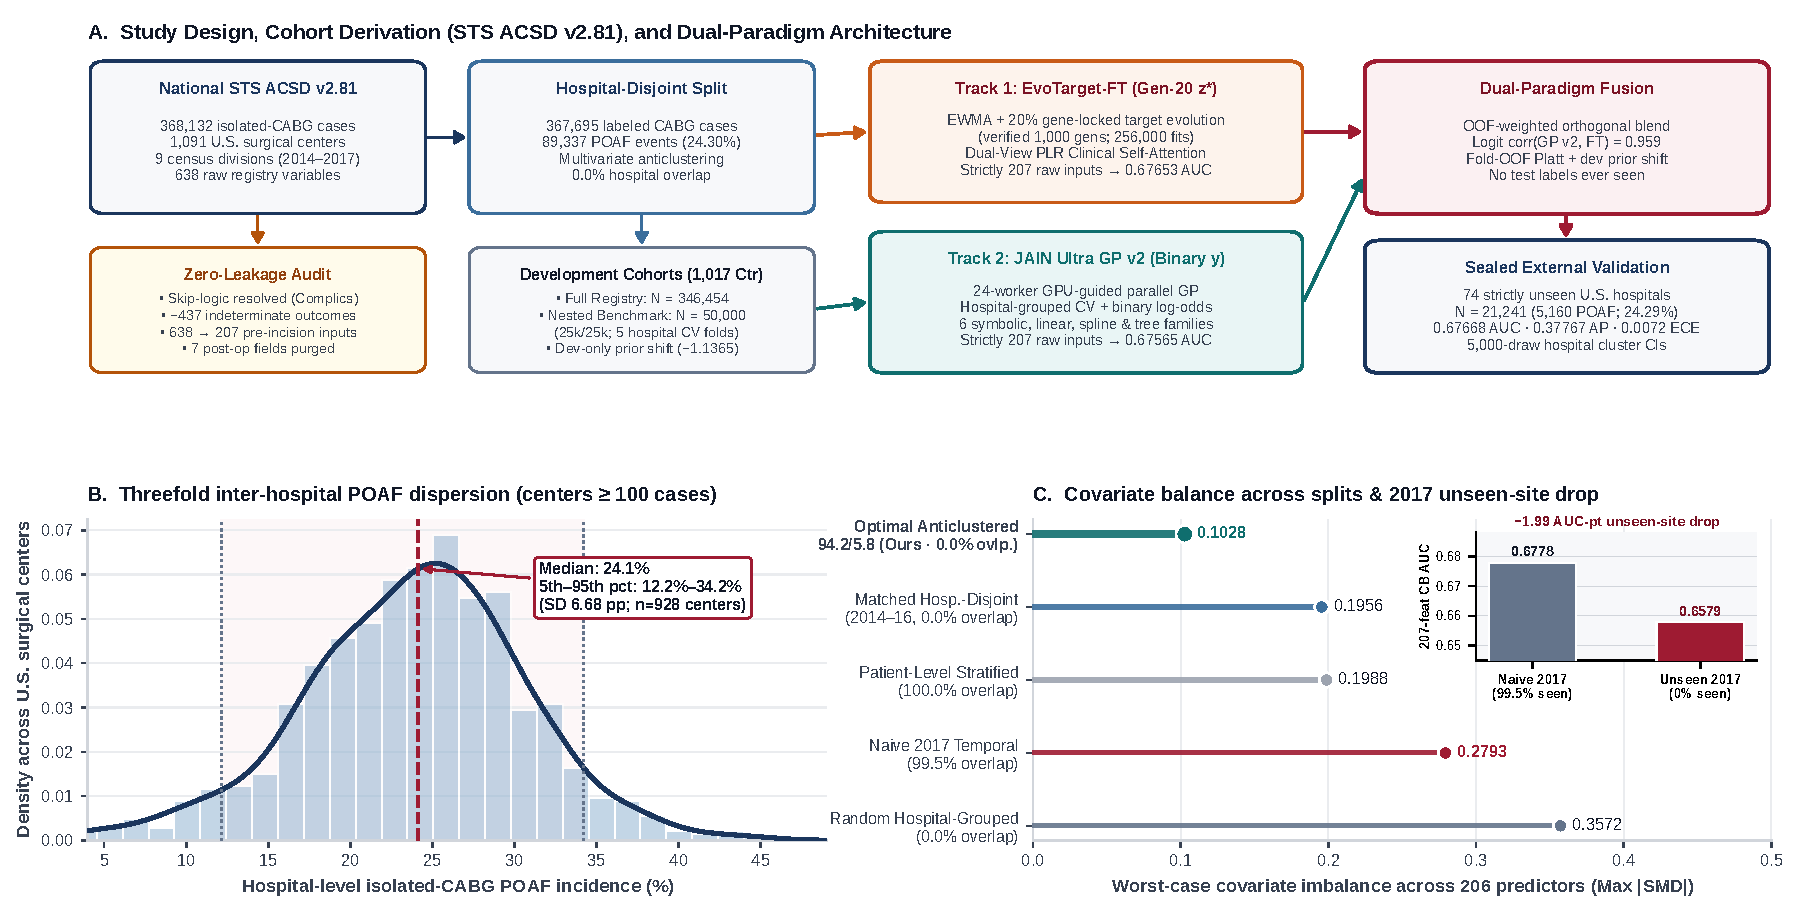
\includegraphics[width=0.90\textwidth]{figures/fig1_study_design_and_split_audit.pdf}
  \caption{\ct{Study Architecture, National STS ACSD v2.81 Cohort Derivation, and Split-Geometry Pathology.} \textbf{A},~Cohort derivation from 368,132 isolated-CABG procedures across 1,091 U.S.\ surgical centers through zero-leakage skip-logic and pre-incision variable auditing into strictly hospital-disjoint external validation (74 unseen hospitals) and the dual-paradigm modeling pipeline (EvoTarget-FT $+$ JAIN Ultra GP v2). \textbf{B},~Threefold dispersion in hospital-level POAF incidence across 928 U.S.\ centers with $\ge 100$ cases (median 24.1\%; 5th--95th percentile 12.2\%--34.2\%; SD 6.68 percentage points). \textbf{C},~Worst-case covariate imbalance ($\mathrm{Max}\,|\mathrm{SMD}|$) across 206 pre-incision predictors for five split designs; inset shows the $-1.99$ AUC-point decline of an identical 207-feature CatBoost model between naive calendar-2017 holdout (99.5\% seen hospitals, 0.6778) and 2017 patients treated at strictly unseen hospitals ($n=3{,}555$, 63 centers, 0.6579).}
  \label{fig:study_design}
\end{figure}

% =============================================================================
%  MAIN BODY: TWO-COLUMN NEJM AI IMRaD (INTRODUCTION, METHODS, RESULTS, DISCUSSION)
% =============================================================================
\clearpage
\twocolumn

\section{Introduction}
\label{sec:intro}

Postoperative atrial fibrillation (POAF) complicates roughly one quarter of isolated coronary artery bypass grafting (CABG) operations and is associated with perioperative stroke, prolonged intensive care, readmission, higher expenditure, and reduced long-term survival.\cite{aranki1996predictors,villareal2004,dobrev2019postoperative,caldonazo2023meta,gaudino2023ehj} Targeted preventive measures---including posterior left pericardiotomy,\cite{gaudino2021palacs} prophylactic amiodarone or colchicine, and intensified telemetry\cite{chatterjee2026sts}---reduce POAF risk, yet universal prophylaxis exposes lower-risk patients to avoidable toxicity. Accurate risk stratification \emph{before skin incision} is therefore essential for both clinical trial enrichment and individualized perioperative care.

Yet the cardiac-surgery machine-learning literature displays a stark paradox. Published POAF models advertise areas under the receiver-operating-characteristic curve (ROC-AUCs) from 0.58 to 0.98, whereas two independent PROBAST critical appraisals concluded that over 80\% carry high risk of bias and shrink from a median apparent AUC of 0.71 to a median external AUC of 0.61.\cite{fields2025poaf,lopeztuesta2026poaf} Apparent AUCs above 0.75 almost invariably reflect post-incision or intensive-care predictors,\cite{mathew2004multicenter,magee2007atrial,ma2025noaf,cao2025mimic4} mixed valve-and-CABG cohorts,\cite{mariscalco2014poaf,burgos2021comaf} single-center internal validation,\cite{cho2026poaf} non-registry waveform or multimodal streams,\cite{han2025aiecg,khalpey2026digital} or continuous telemetry rather than registry-coded treated AF.\cite{filardo2017telemetry,perezgrovas2023jaha}

Compounding this comparability gap, national surgical registries expose two deeper methodological pitfalls. First, in the Society of Thoracic Surgeons Adult Cardiac Surgery Database (STS ACSD),\cite{sts2014v281,shahian2018sts,obrien2018sts2} conditional skip logic leaves uncomplicated recoveries blank, early table columns conceal postoperative durations, and default final-year (calendar-2017) holdouts share 99.5\% of hospitals with training. Second, binary $\{0,1\}$ supervision forces models to fit noisy outcomes shaped heavily by unmeasured intraoperative perturbations,\cite{echahidi2008mechanisms,dobrev2019postoperative} trapping gradient-boosted trees and frontier tabular foundation models (TabPFN-3.5,\cite{hollmann2025tabpfn,jaeger2026tabpfn35} KumoTabular-Large v2,\cite{qu2026kumotabular} and TabFM v1.0.0\cite{kong2026tabfm}) inside a narrow band.

We audited all 368,132 isolated-CABG procedures across 1,091 U.S.\ surgical centers in STS ACSD v2.81 to answer three questions: (1)~what is the true pre-incision discrimination, calibration, clinical utility, and equity of bedside risk proxies, boosted trees, and tabular foundation models on strictly unseen hospitals? (2)~Can evolutionary continuous-target learning (\textbf{EvoTarget-FT}), re-engineered parallel genetic programming (\textbf{JAIN Ultra GP v2}), and their orthogonal \textbf{Dual-Paradigm Fusion} break the 50,000-patient binary ceiling without leakage? (3)~How does performance shift from \emph{cold-start unseen hospitals} (0\% overlap) to a controlled \emph{in-network seen-hospital} regime (all 1,091 centers in training) with and without train-only empirical-Bayes institutional calibration?

\section{Methods}
\label{sec:methods}

\subsection{Data Source, Skip-Logic Audit, and Pre-Incision Feature Partition}
We analyzed all 368,132 isolated-CABG operations recorded in STS ACSD version~2.81 between July~1, 2014, and June~30, 2017, spanning 1,091 U.S.\ surgical centers across all nine U.S.\ Census divisions.\cite{sts2014v281,shahian2018sts,obrien2018sts2} This secondary analysis of de-identified national quality-improvement registry data was conducted under institutional Data Use Agreement governance; no patient-level identifiers or re-operation linkages were accessed, and reporting adheres strictly to TRIPOD+AI (Supplementary Table~\ref{tab:supp_tripod}) and PROBAST+AI guidelines.\cite{collins2024tripodai,moons2025probastai}

Before any model development, we performed a forensic three-part data quality and leakage audit (full ledger in Supplementary Section~S1):
\begin{enumerate}
  \item \textbf{Skip-logic outcome reconstruction:} Under STS Sequence~4930, postoperative atrial fibrillation or flutter requiring treatment (\cli{COtAFib}) is populated only when the parent complication gate \cli{Complics == 1}. Uncomplicated surgical courses (\cli{Complics == 2}; 232,783 cases, 63.31\%) leave \cli{COtAFib} structurally missing; dropping missing \cli{COtAFib} rows induces severe collider bias by conditioning on post-surgical complications.\cite{hernan2020causal} Resolving parent--child skip logic yielded \textbf{367,695 labeled procedures} (437 indeterminate records excluded) with \textbf{89,337 POAF events (24.30\%)}. External polarity checks confirmed that POAF-positive patients were 5.3~years older (68.5 vs.\ 63.2~years) and received discharge amiodarone (74.3\% vs.\ 14.7\%) and warfarin (16.5\% vs.\ 1.8\%) markedly more often.
  \item \textbf{Exhaustive 638 $\to$ 207 pre-incision variable audit:} Every column was audited individually against v2.81 data specifications rather than sliced by column index. Naive positional slicing prior to operative approach (\cli{OPApp}) inadvertently retains seven hidden post-incision or operative-duration leaks: \cli{LOS}, \cli{PLOS}, \cli{ORDuration}, \cli{SIDuration}, \cli{SurgtoMort}, \cli{SurgtoRead}, and \cli{SurgtoSternInf}. All seven fields---together with cardiopulmonary bypass and cross-clamp times, discharge therapies, STS risk-calculator outputs, auxiliary complications, and hospital/surgeon identifiers---were permanently excluded, leaving strictly \textbf{207 pre-incision predictors} (206 numeric, ordinal, or binary clinical variables plus 9-level \cli{Region}).
  \item \textbf{Sentinel decoding and preoperative AF sensitivity flag:} Non-monotonic ``Not Documented'' codes (e.g., code~5 on valve regurgitation, codes~5--6 on chronic lung disease) were decoded prior to clinical scoring. Under v2.81 coding, 1,900 cases (0.52\%; 138 in external validation) carried recorded paroxysmal or persistent preoperative AF (\cli{ArrhythAFib} codes~2--3); we retained an explicit sensitivity flag and report primary performance on both the full cohort and the \emph{no recorded preoperative AF} subgroup ($n=21{,}103$).
\end{enumerate}

\subsection{Forensic Critique of Naive 2017 Splits and Dual Evaluation Regimes}
We audited five partition geometries across all 367,695 labeled cases (Figure~\ref{fig:study_design}B--C; Supplementary Section~\ref{supp:schema}). The conventional temporal split---training on 2014--2016 ($N=306{,}143$) and testing on calendar year 2017 ($N=61{,}552$)---fails both as an external-hospital test and as a stationary statistical benchmark for five reasons: (1)~99.5\% hospital overlap (998 of 1,003 hospitals operating in 2017 appear in training; only 5 centers are unseen); (2)~threefold inter-hospital POAF dispersion (12.2\%--34.2\% across 928 centers with $\ge 100$ cases, 5th--95th percentile; overall 11.7\%--34.8\%, SD~6.68--6.97~pp); (3)~half-year boundary asymmetry (v2.81 spans July~2014--June~2017, making 2014 H2-only at 23.69\% POAF vs.\ 2017 H1-only at 24.83\%); (4)~non-stationary missingness drift ($+6.05$~pp on \cli{LVSD}, $+6.04$~pp on \cli{LVEDD}, $+5.60$~pp on \cli{PctStenAM}; $\mathrm{Max}\,|\mathrm{SMD}| = 0.2793$); and (5)~substantial multivariate covariate shift (adversarial classifier AUC 0.6208 overall; 0.5908 hospital-grouped; 0.7661 vs.\ 2014 alone).

To cleanly separate external transportability from in-network institutional deployment, we constructed two rigorously matched primary evaluation regimes using identical sample sizes ($N=21{,}241$ natural-prior holdout; nested $N=50{,}000$ class-balanced development benchmark for frontier tabular foundation models\cite{jaeger2026tabpfn35,qu2026kumotabular,kong2026tabfm}):

\runin{Regime 1: Cold-Start Unseen-Hospital External Validation (0.0\% Hospital Overlap)}
Random hospital-grouped splitting removes site overlap but produces severe finite-cluster imbalance ($\mathrm{Max}\,|\mathrm{SMD}| = 0.3572$, Region TV $= 0.1645$, POAF gap 1.13~pp). We therefore applied cluster-level multivariate anticlustering\cite{papenberg2021anticlustering} minimizing covariate proxy loss plus $50\times$ 32-dimensional whitened SPlit Energy Distance\cite{joseph2022split,szekely2013energy} (monitoring multi-kernel $\mathrm{MMD}^2$\cite{gretton2012kernel}) subject to a $\ge 5{,}000$ holdout event floor. This partitioned the 1,091 centers into \textbf{1,017 development hospitals} ($N=346{,}454$; 94.2\%) and \textbf{74 strictly unseen validation hospitals} ($N=21{,}241$; 5.8\%, 5,160 events, 24.29\%, 0.0\% hospital overlap), cutting Energy Distance 4.1$\times$ ($0.01732 \to 0.00427$) and $\mathrm{Max}\,|\mathrm{SMD}|$ 3.5$\times$ ($0.3572 \to 0.1028$). Inside the exact same 1,017 development hospitals, class-conditional support-point subsampling\cite{joseph2022split} created a balanced 50,000-patient benchmark (25,000 POAF / 25,000 controls across five exact 10,000-row hospital-disjoint CV folds of 203--204 centers each).

\runin{Regime 2: In-Network Seen-Hospital Deployment (100.0\% All-Hospitals-In-Train)}
To directly quantify the effect of hospital familiarity free of calendar confounding and mirror deployment within an established national registry or health system, we constructed a matched \textbf{100.0\% Seen-Hospital} partition across all 367,695 cases in which \emph{every single one of the 1,091 U.S.\ surgical centers} appears in both the full development set ($N=346{,}454$; 1,091/1,091 hospitals) and the nested 50,000-patient balanced training set (1,091/1,091 hospitals; 5 stratified 10,000-row folds), with zero patient overlap and an exact matched natural-prior holdout of $N=21{,}241$ patients across 1,086 seen hospitals (0 unseen hospitals; 24.30\% POAF). On this seen-hospital cohort, we evaluated every algorithm under both (a)~\textbf{patient-only 207 raw predictors} (isolating implicit hospital familiarity) and (b)~\textbf{in-network site-calibrated deployment}, incorporating each hospital's strictly train-only Empirical-Bayes (EB) shrunk historical log-odds deviation $\hat{\delta}_h = \operatorname{logit}\!\big((e_h + m_0\pi)/(n_h + m_0)\big) - \operatorname{logit}(\pi)$ (computed strictly out-of-fold inside training folds; zero test-label contact), both via parameter-free closed-form hierarchical Bayes site-intercept updating ($\operatorname{Platt}_{\mathrm{OOF}} + \text{dev offset} + \hat{\delta}_h$) and native 208-feature retraining.

\subsection{Comparators, Evolutionary Continuous-Target Learning, and Parallel Genetic Programming}
Every 50,000-patient benchmark model consumed strictly the same 207 raw pre-incision variables under a process-wide sealed-label audit hook blocking any test-label access during training or inference.

\runin{Clinical Scores and Six Binary Tabular ELO Baselines}
We evaluated six established clinical comparators calibrated strictly on the 50k development cohort (Mariscalco POAF,\cite{mariscalco2014poaf} Burgos COM-AF,\cite{burgos2021comaf} $\mathrm{CHA_2DS_2\text{-}VASc}$,\cite{lip2010cha2ds2vasc} HATCH,\cite{devos2010hatch} preoperative Mathew JAMA proxy,\cite{mathew2004multicenter} and continuous age alone) alongside six world-leading binary tabular model families:\cite{grinsztajn2022why,erickson2025tabarena} tuned 5-fold \textbf{CatBoost},\cite{prokhorenkova2018catboost} \textbf{LightGBM},\cite{ke2017lightgbm} and \textbf{XGBoost},\cite{chen2016xgboost} plus three frontier zero-shot in-context tabular foundation models---\textbf{PriorLabs TabPFN-3.5} (native 50k context and $5\times 10\text{k}$ bagged),\cite{hollmann2025tabpfn,jaeger2026tabpfn35} \textbf{NVIDIA KumoTabular-Large v2} ($5\times 10\text{k}$ with mandatory 256-row train-only class-orientation guard),\cite{qu2026kumotabular} and \textbf{Google TabFM v1.0.0} ($5\times 10\text{k}$, 80 NNLS estimators).\cite{kong2026tabfm} Full-registry 346,454-case CatBoost served as the 7$\times$ data-scaling reference, and 92 agent-engineered clinical composites were audited independently across both cohort scales (Supplementary Section~S2).

\runin{EvoTarget-FT: 1,000-Generation Target Evolution and Strictly Nested 2$\times$2 Causal Audit}
In Stage~1, an evolutionary particle-swarm solver distills\cite{hinton2015distilling} continuous training targets $z^{(g)} \in [0,1]^{50{,}000}$ strictly inside the development cohort across whole-hospital shuffled multi-family teachers (CatBoost, LightGBM, XGBoost, and L2 Ridge; 256 fits per generation) using exponentially-weighted moving-average (EWMA) step hardening $z^{(g+1)}=(1-\beta_g)z^{(g)}+\beta_g\tilde{z}^{(g)}$ while gene-locking the 20\% most confident consensus cases (full equations in Supplementary Section~S3). We executed 1,000 full generations (256,000 fits) to audit late-stage stability and selected Generation~20 ($z^*$) for Stage~2 training of \textbf{EvoTarget-FT}, a Dual-View Periodic Linear-ReLU (PLR) clinical self-attention transformer\cite{gorishniy2021revisiting,gorishniy2022embeddings} (4 seeds $\times$ 5 folds, top-3 validation SWA,\cite{izmailov2018swa} composite cross-entropy plus pairwise ranking loss) consuming strictly 207 raw predictors. To resolve any concern regarding global outer-fold target search or 289$\to$207 teacher-feature asymmetry, we also executed a \textbf{strictly nested 5-fold outer-loop} Gen-20 evolution using strictly 207 raw predictors inside each fold's $\sim$814 training hospitals alongside a global 207-raw control, forming an exact 2$\times$2 causal decomposition.

\runin{JAIN Ultra GP v2 and Dual-Paradigm Fusion}
Genetic programming synthesizes explicit symbolic feature pipelines paired with linear, spline, kernel, and tree heads. Profiling default legacy JAIN Ultra uncovered six engineering bottlenecks (single-worker search, 1~GiB worker memory cap, 20,000-row fit cap, random IID internal splits leaking hospital incidence, RMSE fitness on smooth targets, and single-model refits). Our re-engineered build (\textbf{JAIN Ultra GP v2}) resolves all six via 24 parallel GP workers, 8~GiB memory, full 50k training, 64-bin Newton soft-BCE boosting (\cli{histgbm2}) with optional binary-$y$ early stopping (\cli{with\_stop\_target}), hospital-grouped CV optimizing binary ROC-AUC, CUDA learned-ranker guidance, and 64-thread fold-bagging across six evolved operator families (\cli{ensemble}, \cli{winsor\_clip} $\to$ \cli{pair\_ratio} $\to$ \cli{sigmoid} $\to$ \cli{ridge\_gcv}, \cli{pair\_ratio} $\to$ \cli{elasticnet}, \cli{histgbm2}, \cli{oblique\_hinge} $+$ \cli{cheb} $+$ \cli{pair\_prod} $\to$ \cli{ridge}, and \cli{histgbm}). Finally, \textbf{Dual-Paradigm Fusion} blends OOF-weighted log-odds from JAIN Ultra GP v2 and EvoTarget-FT strictly via development OOF optimization.

\subsection{Calibration, Statistical Inference, Clinical Utility, and Equity Analysis}
All 50,000-patient models trained on balanced 50/50 data were mapped back to natural clinical prevalence using uniform fold-OOF Platt scaling\cite{platt1999probabilistic} plus the closed-form strictly development-only Bayes prior-shift offset:\cite{king2001logistic,saerens2002adjusting}
\begin{equation}
  \operatorname{logit}\!\bigl(\hat{p}_{\mathrm{nat}}(x)\bigr) = \operatorname{logit}\!\bigl(\hat{p}_{\mathrm{bal}}(x)\bigr) - 1.136479,
  \label{eq:bayes_shift}
\end{equation}
where $1.136479 = \operatorname{logit}(0.50) - \operatorname{logit}(0.242967)$ uses strictly the development full-training prevalence ($-1.136495$ in the seen-hospital split). Calibration was assessed via 15-bin Expected Calibration Error (ECE),\cite{guo2017calibration,vancalster2019calibration} Integrated Calibration Index (ICI),\cite{austin2019ici} logistic calibration slope, calibration-in-the-large (O:E ratio), Brier score, and decile risk plots.

Because patients cluster within hospitals, all 95\% confidence intervals and paired model comparisons used \textbf{5,000-draw whole-hospital cluster bootstrapping}\cite{davison1997bootstrap,obuchowski1997clustered} (seed~42) resampling all 74 unseen hospitals (Regime~1) or all 1,086 seen hospitals (Regime~2) as intact clusters. Clinical utility was quantified via Decision Curve Analysis (Net Benefit and net unnecessary prophylactic interventions avoided per 100 patients across threshold probabilities 10\%--45\%).\cite{vickers2006decision} Equity and transportability were audited across 25 prespecified demographic, clinical, acuity, and hospital-volume strata, 74 individual hospital funnels, and chronological prospective site-onboarding recalibration (2014--2016 $\to$ 2017). Clinical face validity was evaluated via standardized multivariable surrogate regression ($R^2$ on champion log-odds).

\section{Results}
\label{sec:results}

\subsection{Cohort Characteristics, Data Audit, and Split-Geometry Findings}
Of 368,132 isolated-CABG procedures across 1,091 U.S.\ centers, skip-logic resolution yielded \textbf{367,695 labeled procedures} (437 excluded) with \textbf{89,337 treatment-requiring POAF events (24.30\%)}. Baseline clinical, procedural, and outcome profiles were tightly balanced between full development (1,017 hospitals, $N=346{,}454$, POAF 24.30\%) and strictly unseen external validation (74 centers, $N=21{,}241$, 5,160 events, POAF 24.29\%, 0.0\% overlap; Table~\ref{tab:cohort_baseline}), with $|\mathrm{SMD}| < 0.10$ across every baseline feature and all nine U.S.\ Census divisions matching within 0.18~pp.

\begin{table*}[t]
\centering
\tablefont
\caption{\ct{Baseline Patient, Clinical, Procedural, and Outcome Characteristics Across the National STS ACSD v2.81 Cohorts (1,091 U.S.\ Surgical Centers, 2014--2017).}}
\label{tab:cohort_baseline}
\setlength{\tabcolsep}{5.0pt}
\renewcommand{\arraystretch}{1.04}
\begin{tabularx}{\textwidth}{@{}Yrrrr@{}}
\toprule
\thd{Characteristic} & \thd{Full Development} & \thd{Nested 50k Benchmark} & \thd{Unseen External Test} & \thd{SMD$^{\dagger}$} \\
 & \thd{($N=346{,}454$; 1,017 ctr)} & \thd{($N=50{,}000$; 1,017 ctr)} & \thd{($N=21{,}241$; 74 ctr)} & \thd{(Dev vs.\ Test)} \\
\midrule
\multicolumn{5}{@{}l}{\textit{Demographics and Anthropometry}} \\
\quad Age, mean $\pm$ SD, yr & 65.1 $\pm$ 10.1 & 66.4 $\pm$ 10.0 & 65.2 $\pm$ 10.1 & 0.009 \\
\quad Female sex & 87,423 (25.2\%) & 12,093 (24.2\%) & 5,172 (24.4\%) & 0.020 \\
\quad White race & 285,838 (82.5\%) & 41,977 (84.0\%) & 17,206 (81.0\%) & 0.039 \\
\quad Black race & 26,750 (7.7\%) & 3,413 (6.8\%) & 1,822 (8.6\%) & 0.031 \\
\quad Asian race & 11,889 (3.4\%) & 1,648 (3.3\%) & 842 (4.0\%) & 0.028 \\
\quad Hispanic or Latino ethnicity & 26,921 (7.8\%) & 3,583 (7.2\%) & 1,433 (6.8\%) & 0.039 \\
\quad Body-mass index, mean $\pm$ SD, kg/m$^2$ & 30.1 $\pm$ 6.0 & 30.1 $\pm$ 6.0 & 30.0 $\pm$ 6.0 & 0.014 \\
\quad Body surface area, mean $\pm$ SD, m$^2$ & 2.01 $\pm$ 0.24 & 2.02 $\pm$ 0.24 & 2.01 $\pm$ 0.24 & 0.008 \\
\addlinespace[3pt]
\multicolumn{5}{@{}l}{\textit{Preoperative Clinical Comorbidities and Cardiac Substrate}} \\
\quad Hypertension & 306,810 (88.6\%) & 44,569 (89.1\%) & 19,032 (89.6\%) & 0.033 \\
\quad Diabetes mellitus & 168,522 (48.6\%) & 24,025 (48.0\%) & 10,456 (49.2\%) & 0.012 \\
\quad Heart failure (current or prior) & 75,070 (21.7\%) & 11,333 (22.7\%) & 5,018 (23.6\%) & 0.047 \\
\quad NYHA class III or IV & 35,307 (10.2\%) & 5,449 (10.9\%) & 2,511 (11.8\%) & 0.052 \\
\quad Prior myocardial infarction & 180,339 (52.0\%) & 26,134 (52.3\%) & 10,960 (51.6\%) & 0.009 \\
\quad Chronic lung disease & 82,357 (23.8\%) & 12,200 (24.4\%) & 4,643 (21.9\%) & 0.045 \\
\quad Peripheral vascular disease & 46,703 (13.5\%) & 7,052 (14.1\%) & 2,688 (12.7\%) & 0.025 \\
\quad Cerebrovascular disease & 68,057 (19.6\%) & 10,323 (20.6\%) & 3,959 (18.6\%) & 0.025 \\
\quad Chronic kidney disease (eGFR $<60$) & 72,267 (20.9\%) & 11,068 (22.1\%) & 4,561 (21.5\%) & 0.015 \\
\quad Preoperative dialysis & 9,939 (2.9\%) & 1,435 (2.9\%) & 612 (2.9\%) & 0.001 \\
\quad Recorded preoperative AF history & 1,762 (0.5\%) & 282 (0.6\%) & 138 (0.7\%) & 0.018 \\
\quad Left ventricular EF, mean $\pm$ SD, \% & 52.4 $\pm$ 12.2 & 52.3 $\pm$ 12.3 & 52.4 $\pm$ 12.1 & 0.001 \\
\quad Serum creatinine, mean $\pm$ SD, mg/dL & 1.18 $\pm$ 1.06 & 1.19 $\pm$ 1.06 & 1.20 $\pm$ 1.10 & 0.018 \\
\quad CKD-EPI 2021 eGFR, mL/min/1.73\,m$^2$ & 77.7 $\pm$ 23.5 & 76.5 $\pm$ 23.4 & 77.1 $\pm$ 23.6 & 0.025 \\
\addlinespace[3pt]
\multicolumn{5}{@{}l}{\textit{Surgical Acuity, Anatomy, and Preoperative Medications}} \\
\quad Three-vessel coronary disease & 264,116 (76.2\%) & 38,363 (76.7\%) & 16,465 (77.5\%) & 0.031 \\
\quad Elective operative status & 129,234 (37.3\%) & 18,690 (37.4\%) & 7,887 (37.1\%) & 0.004 \\
\quad Urgent operative status & 202,366 (58.4\%) & 29,130 (58.3\%) & 12,439 (58.6\%) & 0.003 \\
\quad Emergent or salvage status & 14,810 (4.3\%) & 2,173 (4.3\%) & 910 (4.3\%) & 0.001 \\
\quad Preoperative $\beta$-blocker therapy & 312,486 (90.2\%) & 45,027 (90.0\%) & 18,507 (87.1\%) & 0.097 \\
\quad Preoperative amiodarone therapy & 21,722 (6.3\%) & 2,935 (5.9\%) & 1,120 (5.3\%) & 0.043 \\
\addlinespace[3pt]
\multicolumn{5}{@{}l}{\textit{Primary Outcome (Treatment-Requiring New-Onset POAF)}} \\
\quad \textbf{POAF events (STS \texttt{COtAFib})} & \textbf{84,177 (24.30\%)} & \textbf{25,000 (50.0\%)} & \textbf{5,160 (24.29\%)} & \textbf{0.0002} \\
\bottomrule
\end{tabularx}
\par\smallskip\raggedright\fontsize{7.5}{9.4}\selectfont\color{sub}
$^{\dagger}$Standardized mean difference (SMD) comparing the natural-prior full development cohort (1,017 hospitals) with the strictly hospital-disjoint unseen external validation cohort (74 hospitals; 0.0\% hospital overlap). Every clinical characteristic exhibits $|\mathrm{SMD}| < 0.10$, and all nine U.S.\ Census divisions match within 0.18 percentage points. The nested 50,000-patient benchmark is class-balanced (25,000 POAF / 25,000 controls) strictly within the same 1,017 development hospitals and recalibrated back to natural clinical prevalence using the development-only Bayes offset ($-1.1365$).
\end{table*}


Center-level POAF incidence varied nearly threefold across 928 centers with $\ge 100$ cases, spanning 12.2\% to 34.2\% (5th--95th percentile; median 24.1\%, SD~6.68~pp; Figure~\ref{fig:study_design}B). Default calendar-2017 splitting ($N=61{,}552$, 99.5\% hospital overlap) masked severe transport error: an identical 207-feature CatBoost model scored 0.6778 on default 2017 cases yet dropped $-1.99$ AUC points to \textbf{0.6579} on 2017 operations at strictly unseen hospitals ($n=3{,}555$, 63 centers; Figure~\ref{fig:study_design}C). Multivariate anticlustering eliminated overlap while cutting worst-case covariate imbalance 3.5-fold ($\mathrm{Max}\,|\mathrm{SMD}|$: $0.3572 \to 0.1028$) and 32-D Energy Distance 4.1-fold ($0.01732 \to 0.00427$).

\subsection{Primary Unseen-Hospital Validation vs.\ Bedside Proxies and Frontier AI}
Across 74 strictly unseen hospitals ($N=21{,}241$, 207 raw predictors; Table~\ref{tab:primary_results}; Figure~\ref{fig:primary_benchmark}), reconstructed bedside risk proxies showed modest calibrated discrimination (0.5737 for HATCH to 0.6190 for Mariscalco POAF and 0.6451 for preoperative Mathew proxy), whereas all six 50,000-patient binary AI families compressed within a 35-bp plateau from 0.6712 (TabFM) to 0.6746 (Binary FT-Transformer).

\begin{table*}[t]
\centering
\tablefont
\caption{\ct{Primary External Validation Across 74 Strictly Unseen U.S.\ Surgical Centers ($N=21{,}241$; 5,160 POAF Events; 207 Raw Pre-Incision Predictors).}}
\label{tab:primary_results}
\setlength{\tabcolsep}{3.0pt}
\renewcommand{\arraystretch}{1.04}
\begin{tabularx}{\textwidth}{@{}L{1.45cm}Yrrrrrrr@{}}
\toprule
\thd{Class} & \thd{Model / Clinical Proxy} & \thd{ROC-AUC (95\% CI)} & \thd{AP} & \thd{ECE} & \thd{Slope} & \thd{O:E} & \thd{D10 Lift} & \thd{Fusion $\Delta$ bps (95\% CI)} \\
\midrule
\multicolumn{9}{@{}l}{\textit{Reconstructed Bedside Clinical Risk Score Proxies (Calibrated on 50k Development Set)}} \\
Clinical & HATCH Score (proxy) & 0.5737 (0.5640--0.5839) & 0.2872 & 0.0060 & 1.006 & 0.994 & 1.45$\times$ & +1029.3 [+953.5, +1109.9]$^{\ast}$ \\
Clinical & $\mathrm{CHA_2DS_2\text{-}VASc}$ Score (proxy) & 0.5753 (0.5658--0.5845) & 0.2835 & 0.0058 & 1.084 & 0.996 & 1.33$\times$ & +1013.5 [+927.2, +1105.0]$^{\ast}$ \\
Clinical & Burgos COM-AF Score (proxy) & 0.5760 (0.5659--0.5863) & 0.2843 & 0.0068 & 1.067 & 0.993 & 1.38$\times$ & +1006.3 [+927.3, +1095.3]$^{\ast}$ \\
Clinical & Mariscalco POAF Score (proxy) & 0.6190 (0.6102--0.6281) & 0.3097 & 0.0190 & 0.962 & 1.004 & 1.67$\times$ & +577.0 [+495.6, +656.9]$^{\ast}$ \\
Clinical & Continuous Age Alone & 0.6397 (0.6292--0.6503) & 0.3367 & 0.0127 & 0.955 & 0.996 & 1.61$\times$ & +369.6 [+290.4, +449.0]$^{\ast}$ \\
Clinical & Preoperative Mathew Proxy & 0.6451 (0.6344--0.6558) & 0.3435 & 0.0097 & 0.965 & 0.997 & 1.63$\times$ & +316.1 [+245.1, +386.1]$^{\ast}$ \\
\midrule
\multicolumn{9}{@{}l}{\textit{World-Leading Binary Tabular Foundation Models and GBDTs ($N=50{,}000$, 207 Raw Predictors)}} \\
Tabular FM & Google TabFM v1.0.0 (5$\times$10k) & 0.6712 (0.6628--0.6805) & 0.3697 & 0.0090 & 0.963 & 0.992 & 1.78$\times$ & +55.3 [+28.6, +81.5]$^{\ast}$ \\
Tabular FM & NVIDIA KumoTabular-L v2 (5$\times$10k) & 0.6715 (0.6632--0.6807) & 0.3693 & 0.0070 & 1.040 & 1.004 & 1.79$\times$ & +52.0 [+21.6, +83.3]$^{\ast}$ \\
GBDT & XGBoost (5-fold tuned) & 0.6736 (0.6658--0.6824) & 0.3722 & 0.0069 & 0.998 & 0.992 & 1.81$\times$ & +31.1 [+11.7, +49.4]$^{\ast}$ \\
GBDT & LightGBM (5-fold tuned) & 0.6736 (0.6657--0.6826) & 0.3725 & 0.0060 & 1.003 & 0.993 & 1.80$\times$ & +30.5 [+11.3, +48.0]$^{\ast}$ \\
Tabular FM & PriorLabs TabPFN-3.5 (50k native) & 0.6738 (0.6659--0.6827) & 0.3728 & 0.0068 & 1.002 & 1.002 & 1.83$\times$ & +29.2 [+8.2, +53.5]$^{\ast}$ \\
GBDT & CatBoost (5-fold binary ref) & 0.6742 (0.6659--0.6835) & 0.3744 & 0.0078 & 1.056 & 1.001 & 1.84$\times$ & +24.5 [+7.2, +42.2]$^{\ast}$ \\
Neural & Binary FT-Transformer (Gen-0) & 0.6746 (0.6664--0.6838) & 0.3756 & 0.0054 & 1.026 & 0.996 & 1.84$\times$ & +20.3 [+2.4, +38.2]$^{\ast}$ \\
\midrule
\multicolumn{9}{@{}l}{\textit{Proposed Evolutionary Target Learning, Parallel GP, and Dual-Paradigm Fusion ($N=50{,}000$, 207 Raw)}} \\
Evolved Tree & CatBoost CE (Gen-20 $z^*$) & 0.6754 (0.6673--0.6844) & 0.3750 & 0.0084 & 0.957 & 0.995 & 1.85$\times$ & +13.0 [-2.2, +26.7] \\
Parallel GP & JAIN Ultra GP v2 (6-family binary) & 0.6756 (0.6673--0.6850) & 0.3758 & 0.0080 & 1.002 & 0.991 & 1.85$\times$ & +10.3 [-5.6, +25.8] \\
Nested $z^*$ & EvoTarget-FT (Strictly Nested 207) & 0.6759 (0.6678--0.6851) & 0.3764 & 0.0074 & 1.008 & 0.995 & 1.86$\times$ & +8.0 [+1.0, +15.3]$^{\ast}$ \\
Gen-0 Blend & Fair Fusion (GP v2 $+$ Binary FT) & 0.6762 (0.6681--0.6854) & 0.3767 & 0.0046 & 1.012 & 0.993 & 1.84$\times$ & +4.5 [-4.2, +13.2] \\
Evolved Attn & EvoTarget-FT (Gen-20 $z^*$) & 0.6765 (0.6685--0.6856) & 0.3775 & 0.0085 & 0.976 & 0.996 & 1.85$\times$ & +1.4 [-4.0, +6.9] \\
\rowcolor{primarytint} \textbf{Champion} & \textbf{Dual-Paradigm Fusion (GP v2 $+$ FT)} & \textbf{0.6767 (0.6686--0.6858)} & \textbf{0.3777} & \textbf{0.0072} & \textbf{0.983} & \textbf{0.994} & \textbf{1.84$\times$} & \textbf{Reference} \\
\midrule
\multicolumn{9}{@{}l}{\textit{Full National Registry Data-Scale Reference ($7\times$ Larger Training Cohort, $N=346{,}454$)}} \\
7$\times$ Ref & CatBoost Full Registry (346k, 207 raw) & 0.6773 (0.6695--0.6862) & 0.3776 & 0.0076 & 1.023 & 1.000 & 1.84$\times$ & -6.4 [-23.0, +10.5] \\
\bottomrule
\end{tabularx}
\par\smallskip\raggedright\fontsize{7.3}{9.1}\selectfont\color{sub}
All models consume strictly the same 207 raw pre-incision predictors (reconstructed STS pre-incision proxies for bedside scores) and are calibrated to natural prevalence via fold-OOF Platt scaling plus the development-only Bayes offset ($-1.1365$; zero test-label contact). Intervals reflect 5,000 whole-hospital cluster bootstrap draws across all 74 unseen centers conditional on retrospective evaluation. $^{\ast}$95\% cluster CI strictly excludes zero. Dual-Paradigm Fusion recovers 79.2\% of the 7$\times$ 50k$\to$346k CatBoost gap while exceeding 346k CatBoost in AP (0.3777 vs.\ 0.3776), ECE (0.0072 vs.\ 0.0076), 2017 unseen-hospital AUC (0.6579 vs.\ 0.6578), and rare clinical tails (0.6935 vs.\ 0.6928), and strictly outperforming a 3-way binary neural--GBDT--TabPFN blend ($+9.9$ bps $[+0.6, +19.7]$).
\end{table*}


\begin{figure*}[t]
  \centering
  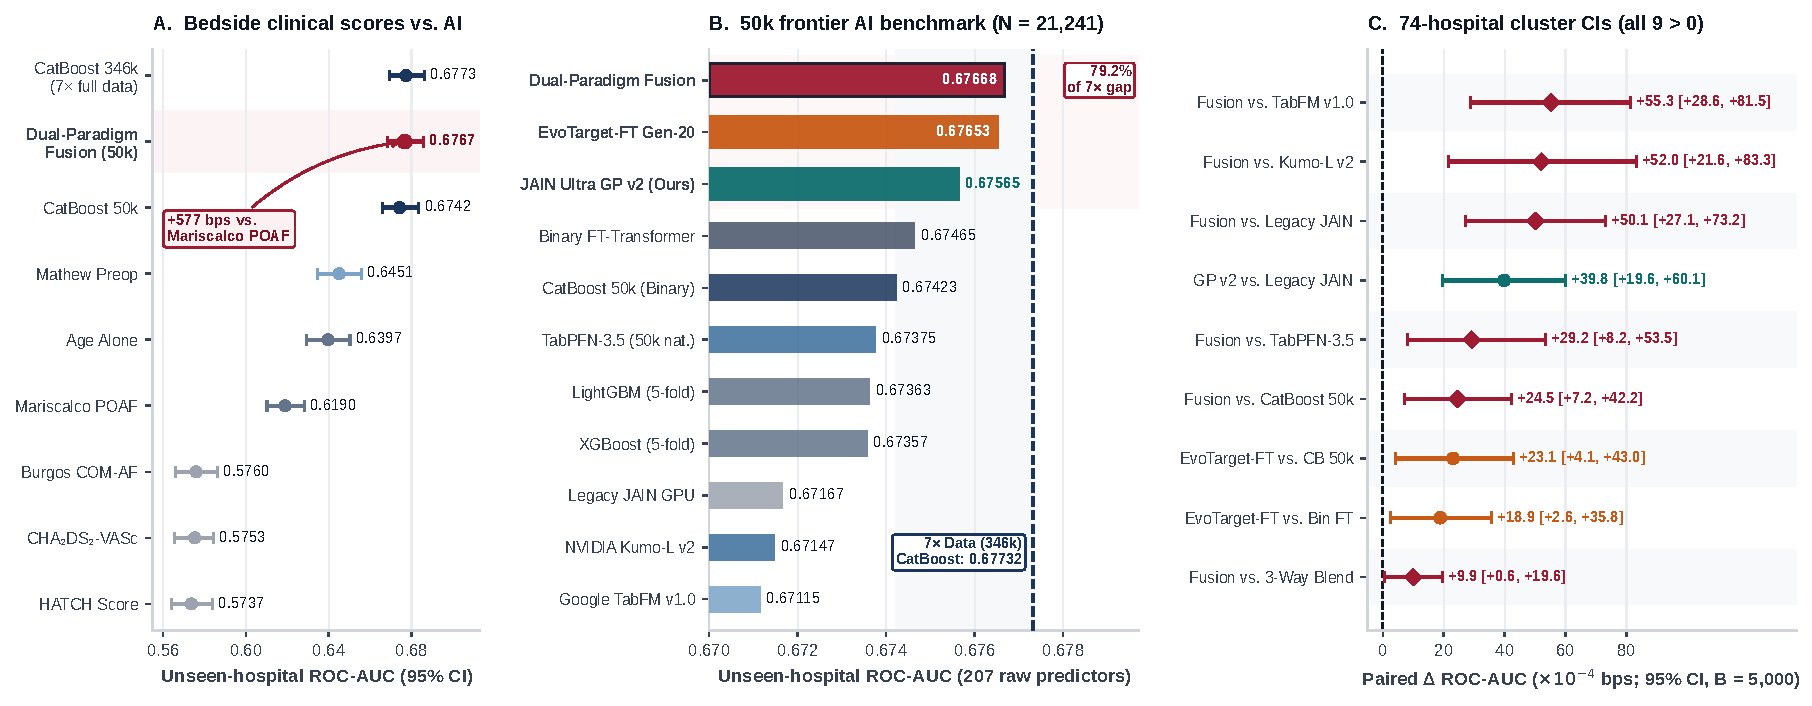
\includegraphics[width=\textwidth]{figures/fig2_primary_benchmark_and_forest.pdf}
  \caption{\ct{Primary Unseen-Hospital External Validation ($N=21{,}241$, 74 Unseen U.S.\ Hospitals, 207 Raw Pre-Incision Predictors).} \textbf{A},~Head-to-head ROC-AUC across six calibrated bedside clinical proxies, six world-leading 50k binary tabular model families, the proposed evolutionary and parallel-GP models, and the 7$\times$-larger 346k national full-registry CatBoost reference. \textbf{B},~Paired 5,000-draw 74-hospital cluster bootstrap contrasts ($\Delta$ ROC-AUC in basis points, $\times 10^{-4}$); filled diamonds indicate 95\% CIs strictly excluding zero. Dual-Paradigm Fusion outperforms every bedside proxy and every 50k binary baseline, including a 3-way binary neural--GBDT--TabPFN blend ($+9.9$ bps $[+0.6, +19.7]$).}
  \label{fig:primary_benchmark}
\end{figure*}

Both proposed paradigms broke above the 50k binary ceiling on identical 207 raw predictors: \textbf{JAIN Ultra GP v2} reached 0.6756 (95\% CI, 0.6673--0.6850), \textbf{EvoTarget-FT} (Gen-20 $z^*$) reached 0.6765 (0.6685--0.6856), and \textbf{Dual-Paradigm Fusion} achieved \textbf{0.6767 (0.6686--0.6858; AP~0.3777; ECE~0.0072; top-decile lift 1.84$\times$)}. Under 5,000-draw 74-hospital cluster bootstrapping (Table~\ref{tab:primary_results}; Figure~\ref{fig:primary_benchmark}B), Fusion decisively surpassed every bedside proxy---including $+577.0$ bps ($[+495.6, +656.9]$) over Mariscalco POAF and $+316.1$ bps over Mathew proxy---and outperformed every 50k binary AI baseline with 95\% cluster CIs strictly $>0$: $+55.3$ bps over TabFM, $+52.0$ bps over KumoTabular-Large, $+50.1$ bps over legacy JAIN GPU, $+31.1$ bps over XGBoost, $+30.5$ bps over LightGBM, $+29.2$ bps over TabPFN-3.5, $+24.5$ bps over CatBoost 50k, $+20.3$ bps over Binary FT, and $+9.9$ bps ($[+0.6, +19.7]$, $P>0=0.982$) over a 3-way binary blend (0.6757). Relative to 7$\times$-larger 346k CatBoost (0.6773), 50k Fusion recovered \textbf{79.2\%} of the scaling gap while surpassing 346k CatBoost in AP (0.3777 vs.\ 0.3776), ECE (0.0072 vs.\ 0.0076), 2017 unseen hospitals (0.6579 vs.\ 0.6578), and rare clinical tails (0.6935 vs.\ 0.6928), with identical performance excluding recorded preoperative AF ($n=21{,}103$; AUC~0.6771).

\subsection{1,000-Generation Target Evolution and Strictly Nested 2$\times$2 Causal Proof}
Tracking Stage-1 target evolution through 1,000 generations (256,000 fits; Figure~\ref{fig:target_evolution}A) confirmed rapid early denoising and asymptotic stability without collapse: EvoTarget-FT climbed from 0.67465 (Gen~0) to \textbf{0.67654} at Gen~20 ($+18.9$ bps $[+2.6, +35.8]$) and plateaued cleanly at 0.67592 through Gen~1,000 (CatBoost CE: $0.67408 \to 0.67538$ at Gen~20 $\to 0.67511$ at Gen~1,000). Replacing binary labels with Gen-20 continuous targets $z^*$ lifted unseen-hospital discrimination across \textbf{all seven independent architectures} (Figure~\ref{fig:target_evolution}B), with 5 of 7 cluster CIs strictly $>0$, including large gains on zero-shot tabular foundation model regressors: TabFM Reg $+97.2$ bps (beating binary TabFM Cls by $+26.7$ bps $[+3.7, +49.8]$), KumoTabular Reg $+27.9$ bps (beating binary Kumo Cls by $+35.2$ bps $[+9.0, +63.5]$), TabPFN-3.5 $5\times 10\text{k}$ Reg $+26.1$ bps, EvoTarget-FT $+18.9$ bps, and CatBoost $+12.9$ bps.

\begin{figure*}[t]
  \centering
  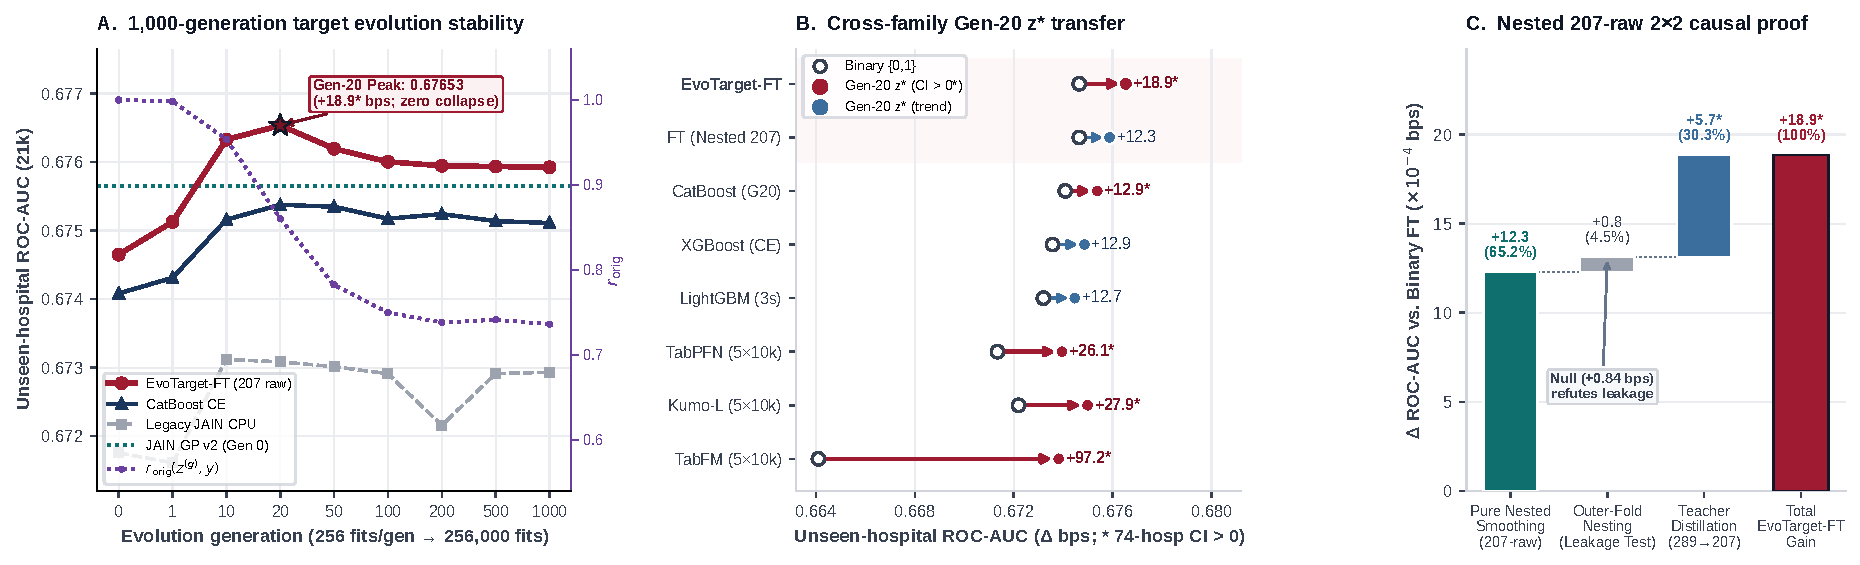
\includegraphics[width=\textwidth]{figures/fig3_target_evolution_and_causal_proof.pdf}
  \caption{\ct{1,000-Generation Target Evolution Stability, Cross-Architecture Transfer, and Strictly Nested 2$\times$2 Causal Audit.} \textbf{A},~External unseen-hospital ROC-AUC across nine milestones from Generation~0 to Generation~1,000 (256,000 cumulative Stage-1 fits), confirming peak discrimination at Gen~20 and a non-collapsing plateau through Gen~1,000. \textbf{B},~Replacing binary $\{0,1\}$ labels with Gen-20 continuous targets ($z^*$) yields positive unseen-hospital lift across all seven distinct tabular model architectures (three tabular foundation models, three GBDTs, and FT-Transformer), with five of seven paired 74-hospital CIs strictly exceeding zero. \textbf{C},~Exact 2$\times$2 causal decomposition separating genuine continuous-target denoising ($+12.3$ bps strictly nested on 207 raw predictors) from negligible outer-fold overlap ($+0.8$ bps, $P=0.68$) and Stage-1 teacher-feature distillation ($+5.7$ bps $[+0.3, +10.6]$).}
  \label{fig:target_evolution}
\end{figure*}

The strictly nested 2$\times$2 causal audit partitioned EvoTarget-FT's $+18.85$-bp gain into three exact mechanisms (Figure~\ref{fig:target_evolution}C): (1)~strictly nested 5-fold outer-loop 207-raw evolution (zero validation-hospital access) delivered \textbf{0.67588} ($+12.29$ bps $[-3.25, +28.53]$, $P>0=0.942$; 65\% of total gain); (2)~moving from nested to global 207-raw search added a statistically null $+0.84$ bps ($[-2.43, +4.40]$), ruling out outer-fold leakage; and (3)~Stage-1 privileged distillation of 82 clinical features into $z^*$ while keeping Stage-2 strictly on 207 raw predictors contributed a cluster-confirmed \textbf{$+5.72$ bps ($[+0.33, +10.61]$)}.

\subsection{JAIN Ultra GP v2 Engineering Rescue and Pre-Incision Physiological Drivers}
Resolving all six legacy JAIN bottlenecks drove a \textbf{$+39.8$-bp external rescue ($[+19.6, +60.1]$, $P>0=0.9998$)} from legacy GPU Gen-20 (0.6717) to the 6-family binary \textbf{JAIN Ultra GP v2} ensemble at \textbf{0.6756} (Figure~\ref{fig:gp_v2_interp}A), outperforming TabFM ($+45.0$ bps) and KumoTabular ($+41.8$ bps) standalone. Binary-$y$ early stopping rescued soft-target GP by $+9.1$ bps ($[+0.5, +18.0]$), while fresh-seed 7-fold hospital CV ($r=0.959$ on binary $y$) exposed $+55$-bp tree-to-tree OOF optimism on global $z^*$ explaining why binary-$y$ GP transported best (Figure~\ref{fig:gp_v2_interp}B). Even at Gen~0 (zero target evolution), blending JAIN Ultra GP v2 with Binary FT achieved 0.6762 with the lowest calibration error overall (ECE~0.0046; $+15.8$ bps $[+1.0, +30.3]$ over Binary FT).

\begin{figure*}[t]
  \centering
  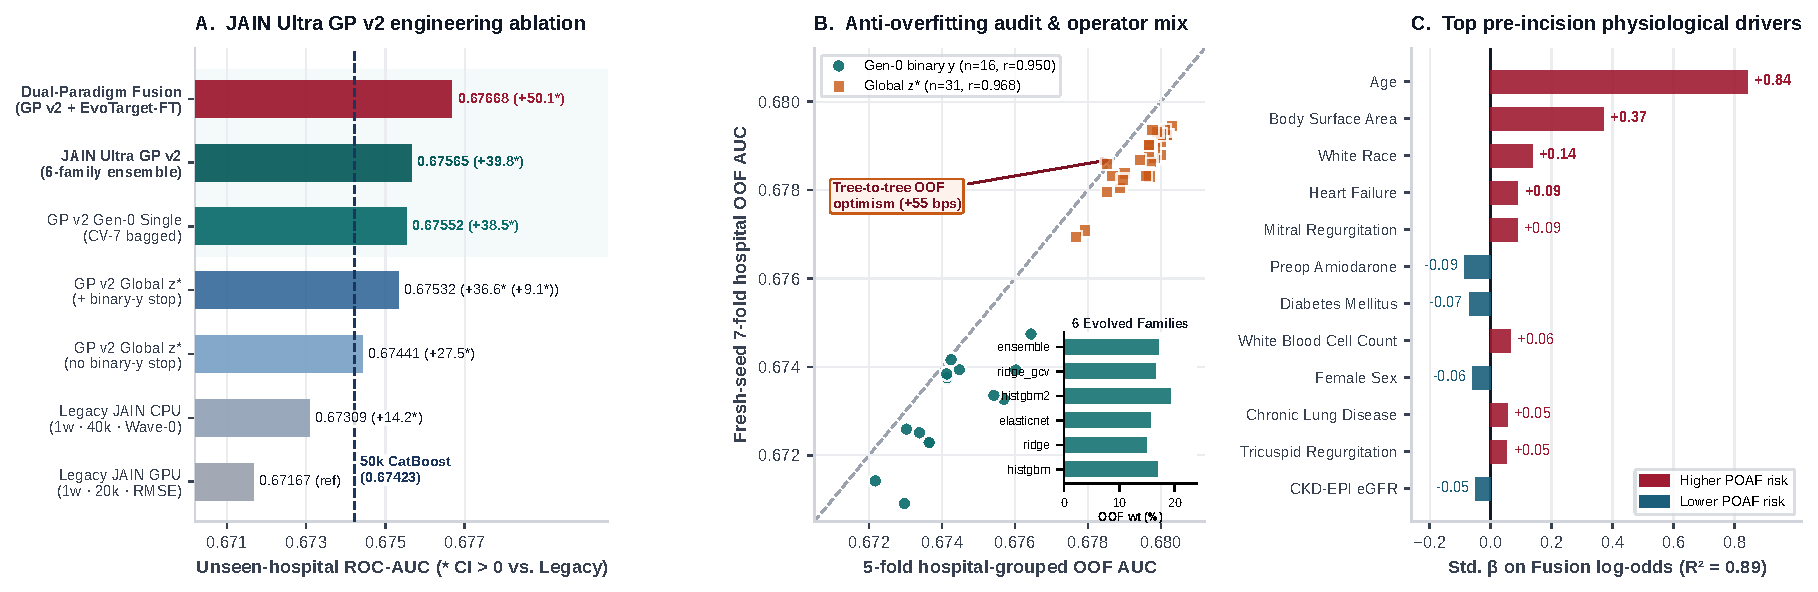
\includegraphics[width=\textwidth]{figures/fig4_jain_gp_v2_and_interpretability.pdf}
  \caption{\ct{JAIN Ultra GP v2 Engineering Rescue, Anti-Overfitting Verification, and Pre-Incision Physiological Drivers.} \textbf{A},~Stepwise external ROC-AUC rescue on 74 unseen hospitals from legacy JAIN GPU (0.6717) to JAIN Ultra GP v2 (0.6756, $+39.8$ bps $[+19.6, +60.1]$) and Dual-Paradigm Fusion (0.6767). \textbf{B},~Fresh-seed 7-fold vs.\ 5-fold hospital-grouped OOF verification across evolved Hall-of-Fame pipelines ($r=0.959$ on binary $y$), exposing $+55$-bp tree-to-tree OOF optimism on global $z^*$ and showing the balanced 6-family symbolic/linear/tree ensemble weights (inset). \textbf{C},~Top 12 standardized multivariable clinical drivers of Dual-Paradigm Fusion log-odds ($R^2 = 0.89$), showing concordant surgical pathophysiology including protective preoperative amiodarone ($\beta = -0.09$).}
  \label{fig:gp_v2_interp}
\end{figure*}

Log-odds from JAIN Ultra GP v2 and EvoTarget-FT correlated strongly yet imperfectly ($r=0.9591$), enabling orthogonal fusion. Standardized multivariable surrogate regression explained \textbf{89.0\%} ($R^2 = 0.8896$) of Dual-Paradigm Fusion log-odds variance with physiologically transparent pre-incision drivers (Figure~\ref{fig:gp_v2_interp}C): advancing age ($\beta=+0.84$), body surface area ($+0.37$), White race ($+0.14$), heart failure ($+0.09$), mitral regurgitation ($+0.09$), white blood cell count ($+0.06$), chronic lung disease ($+0.05$), and tricuspid regurgitation ($+0.05$) increased risk, whereas preoperative amiodarone ($\beta=-0.09$), diabetes ($-0.07$), female sex ($-0.06$), and preserved eGFR ($-0.05$) were independently protective.

\subsection{Calibration, Decile Stratification, and Decision Curve Clinical Utility}
Using development-only recalibration (zero test-label contact), Dual-Paradigm Fusion achieved near-ideal external calibration across 21,241 unseen-hospital cases (Figure~\ref{fig:calibration_dca}A): slope \textbf{0.983}, O:E \textbf{0.994}, 15-bin ECE \textbf{0.0072}, and ICI \textbf{0.0114}. Observed POAF rose monotonically across predicted deciles from \textbf{6.07\%} in D1 to \textbf{44.82\%} in D10---a \textbf{7.4-fold} risk separation with 1.84$\times$ top-decile enrichment (Figure~\ref{fig:calibration_dca}B).

\begin{figure*}[t]
  \centering
  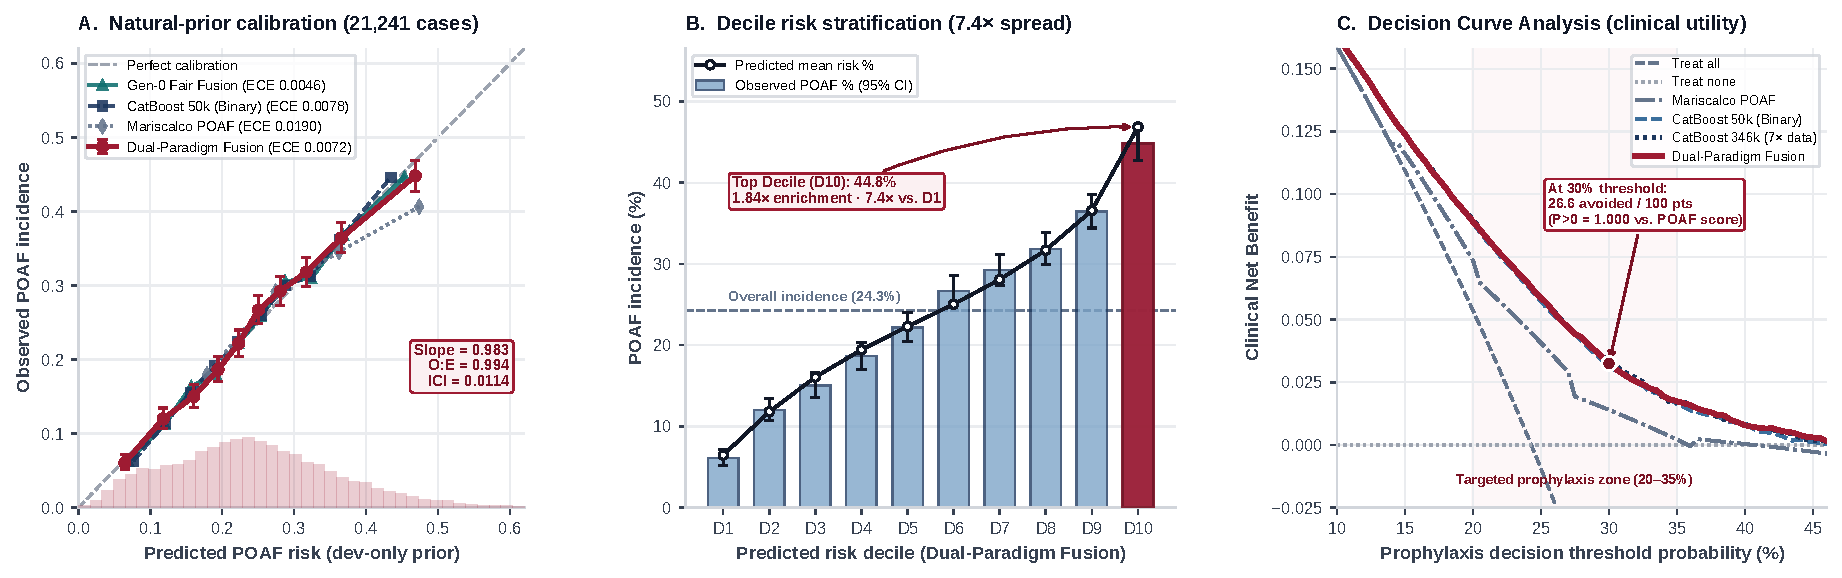
\includegraphics[width=\textwidth]{figures/fig5_calibration_stratification_dca.pdf}
  \caption{\ct{Clinical Calibration, Decile Risk Stratification, and Decision Curve Clinical Utility ($N=21{,}241$, 74 Unseen Hospitals).} \textbf{A},~Natural-prior calibration curves using strictly development-only recalibration (Bayes offset $-1.1365$), showing Dual-Paradigm Fusion alignment across deciles (slope~0.983, O:E~0.994, ECE~0.0072, ICI~0.0114). \textbf{B},~Monotonic risk stratification across predicted deciles from 6.07\% POAF in D1 to 44.82\% in D10 (7.4$\times$ gradient; 1.84$\times$ top-decile enrichment). \textbf{C},~Decision Curve Analysis demonstrating strictly superior Net Benefit across clinically actionable 15\%--40\% prophylaxis thresholds, avoiding 20.4--33.8 unnecessary interventions per 100 patients at 25\%--35\% thresholds ($P>0=1.000$ vs.\ Mariscalco POAF).}
  \label{fig:calibration_dca}
\end{figure*}

In Decision Curve Analysis (Figure~\ref{fig:calibration_dca}C; Supplementary Table~\ref{tab:supp_dca}), Fusion generated strictly positive Net Benefit across 15\%--40\% prophylaxis thresholds. At 25\%, 30\%, and 35\% decision thresholds (flagging 45.1\%, 29.3\%, and 17.5\% of patients), Fusion achieved Net Benefits of \textbf{0.0587}, \textbf{0.0325}, and \textbf{0.0174} (vs.\ negative values for universal prophylaxis), avoiding \textbf{20.4}, \textbf{26.6}, and \textbf{33.8 unnecessary prophylactic interventions per 100 CABG patients} and outperforming Mariscalco POAF across 100\% of hospital-cluster bootstrap draws ($P>0=1.000$).

\subsection{Demographic Equity and 74-Hospital Center Transportability}
Across 25 prespecified demographic, comorbidity, acuity, stress-slice, and hospital-volume strata (Figure~\ref{fig:equity_transport}A; Supplementary Table~\ref{tab:supp_subgroups}), Dual-Paradigm Fusion outperformed Mariscalco POAF in all 25 strata ($+374$ to $+1{,}333$ bps) and beat CatBoost 50k in \textbf{24 of 25 strata} (near-parity $-1.2$ bps in age $<60$~yr), maintaining strong performance across female (0.6891), male (0.6719), Black (0.6849), Hispanic/Latino (0.7146), diabetic (0.6812), LVEF $<40\%$ (0.6787), urgent/emergent (0.6830), rare-tail (0.6935), and low-, mid-, and high-volume center cohorts (0.6818--0.6851).

\begin{figure*}[t]
  \centering
  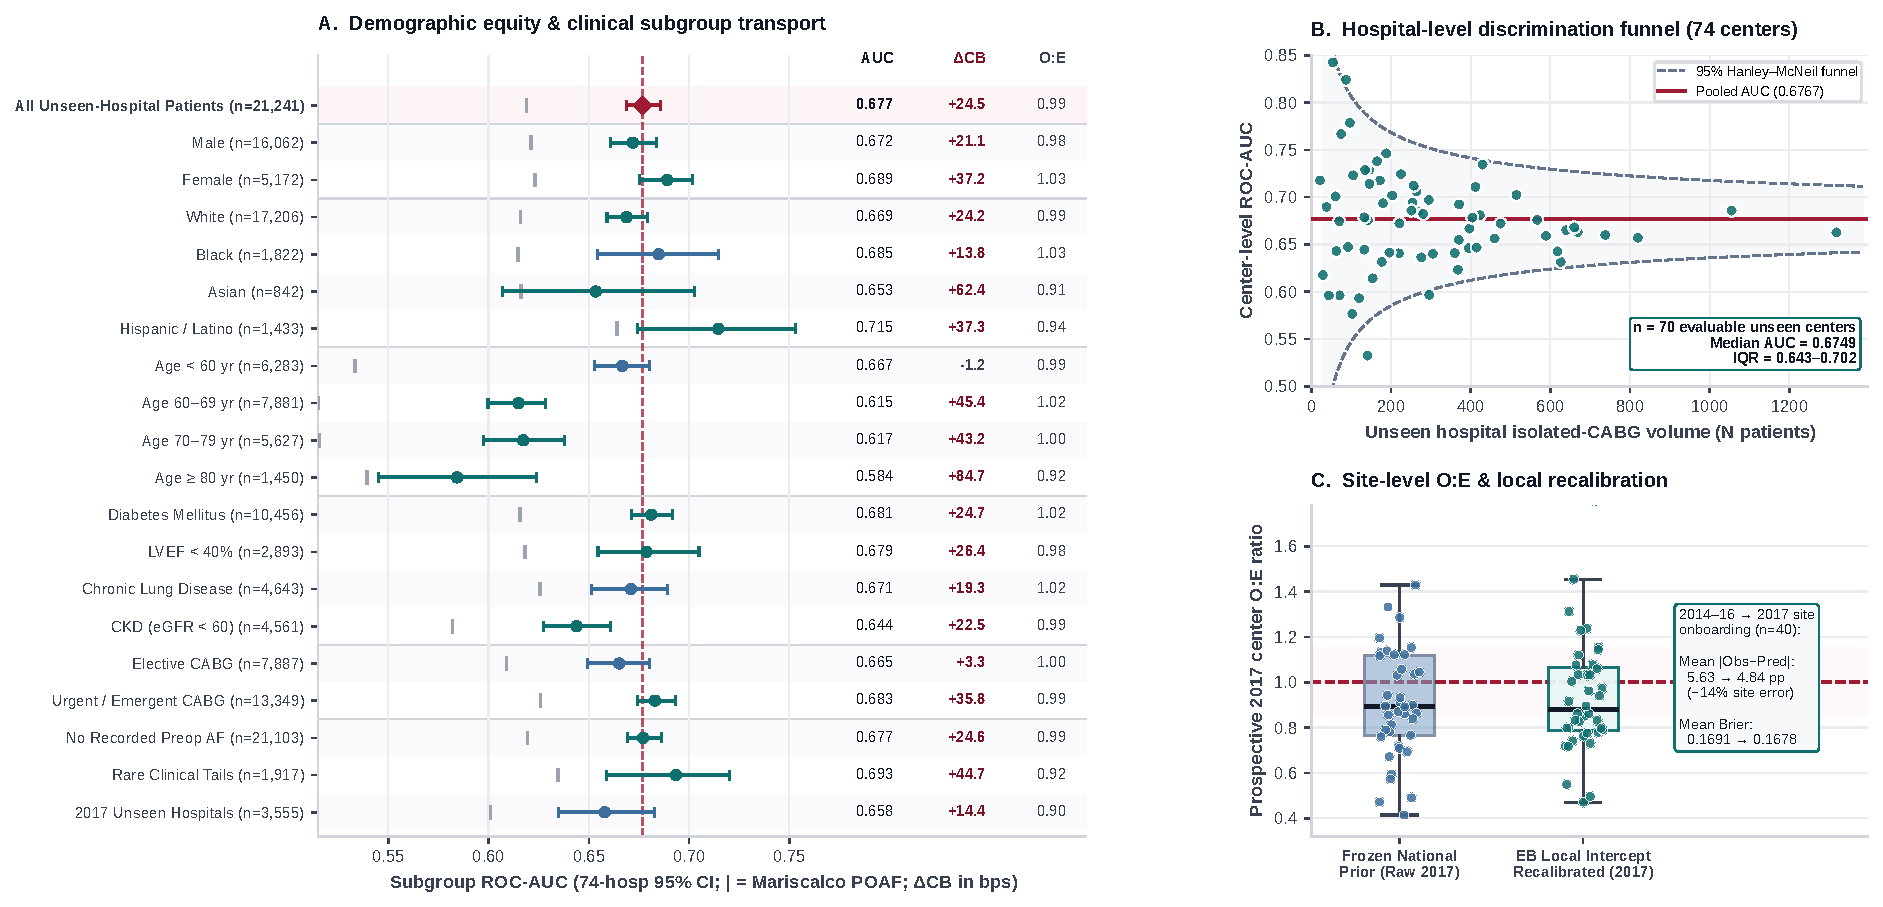
\includegraphics[width=\textwidth]{figures/fig6_equity_subgroups_and_hospital_transport.pdf}
  \caption{\ct{Subgroup Equity Audit, 74-Hospital Discrimination Funnel, and Prospective Local Intercept Recalibration.} \textbf{A},~Subgroup ROC-AUC (74-hospital 95\% CIs), $\Delta$ vs.\ CatBoost 50k (bps), and O:E ratio across demographic, comorbidity, acuity, and stress strata (vertical ticks show Mariscalco POAF). \textbf{B},~Hospital-level ROC-AUC across 70 evaluable unseen centers plotted against case volume within the 95\% Hanley--McNeil funnel (median AUC 0.6749, IQR 0.6434--0.7021). \textbf{C},~Prospective chronological site-onboarding recalibration (2014--2016 onboarding $\to$ 2017 deployment across 40 centers), showing that empirical-Bayes local intercept updating ($m_0=100$) lowers center-level mean absolute POAF rate error by 14\% (5.63 $\to$ 4.84~pp) and improves Brier score (0.1691 $\to$ 0.1678).}
  \label{fig:equity_transport}
\end{figure*}

Across 70 evaluable unseen hospitals, center-level AUCs tracked inside the 95\% Hanley--McNeil funnel (median \textbf{0.6749}, IQR 0.6434--0.7021; Figure~\ref{fig:equity_transport}B), while uncalibrated center O:E ratios reflected site incidence dispersion (median 0.958, IQR 0.856--1.135). In chronological prospective site onboarding (2014--2016 $\to$ 2017 across 40 centers; Figure~\ref{fig:equity_transport}C), updating a single empirical-Bayes local intercept ($m_0=100$) reduced prospective center mean absolute POAF rate error by \textbf{14\%} (5.63 $\to$ 4.84~pp) and improved Brier score (0.1691 $\to$ 0.1678).

\subsection{Seen-Hospital In-Network Deployment vs.\ Cold-Start Transport}
Evaluating every model on the matched \textbf{100.0\% Seen-Hospital} split (all 1,091 hospitals in training; 0 unseen test centers; $N=21{,}241$ holdout across 1,086 seen centers; Table~\ref{tab:seen_vs_unseen}; Figure~\ref{fig:seen_vs_unseen}) isolated hospital familiarity free of calendar confounding and yielded three clear findings.

\begin{table*}[t]
\centering\tablefont
\caption{\ct{Head-to-Head Transport Audit: Unseen-Hospital Cold Start (0\% Overlap, 74 Centers) vs.\ Seen-Hospital In-Network Deployment (100\% Overlap, All 1,091 Centers in Training; $N=21{,}241$ Natural-Prior Holdout).}}
\label{tab:seen_vs_unseen}
\setlength{\tabcolsep}{3.8pt}
\renewcommand{\arraystretch}{1.04}
\begin{tabularx}{\textwidth}{@{}Yrrrrrr@{}}
\toprule
\thd{Model Family} & \thd{Unseen Hosp.} & \thd{Seen Hosp.} & \thd{Seen + 50k} & \thd{Seen + 346k} & \thd{Site-Prior} & \thd{In-Net} \\
 & \thd{(0\% ovlp, 207)} & \thd{(100\%, 207 raw)} & \thd{EB Site Prior} & \thd{EB Site Prior} & \thd{Gain (bps)} & \thd{ECE} \\
\midrule
\multicolumn{7}{@{}l}{\textit{Bedside Clinical Proxy Reference}} \\
Mariscalco POAF Score (proxy) & 0.6190 & 0.6276 & --- & --- & --- & 0.0166 \\
\midrule
\multicolumn{7}{@{}l}{\textit{50,000-Patient Parity Benchmark (207 Raw Predictors $+$ Parameter-Free Closed-Form EB Hospital Priors)}} \\
Google TabFM v1.0.0 (5$\times$10k) & 0.6712 & 0.6775 & 0.6918 & 0.6986 & +210 & 0.0093 \\
NVIDIA KumoTabular-L v2 (5$\times$10k) & 0.6715 & 0.6764 & 0.6911 & 0.6977 & +213 & 0.0080 \\
XGBoost (5-fold binary) & 0.6736 & 0.6774 & 0.6895 & 0.6958 & +184 & 0.0100 \\
LightGBM (5-fold binary) & 0.6736 & 0.6780 & 0.6897 & 0.6960 & +180 & 0.0084 \\
PriorLabs TabPFN-3.5 (50k native) & 0.6738 & 0.6795 & 0.6919 & 0.6982 & +187 & 0.0086 \\
CatBoost 50k (5-fold binary) & 0.6742 & 0.6777 & 0.6902 & 0.6966 & +188 & 0.0089 \\
Binary FT-Transformer (Gen-0) & 0.6746 & 0.6784 & 0.6890 & 0.6958 & +174 & 0.0067 \\
JAIN Ultra GP v2 (6-family) & 0.6756 & 0.6788 & 0.6904 & 0.6969 & +181 & 0.0098 \\
EvoTarget-FT (Gen-20 $z^*$) & 0.6765 & 0.6793 & 0.6906 & 0.6972 & +179 & 0.0117 \\
\rowcolor{primarytint} \textbf{Dual-Paradigm Fusion (GP v2 $+$ FT)} & \textbf{0.6767} & \textbf{0.6794} & \textbf{0.6909} & \textbf{0.6974} & \textbf{+180} & \textbf{0.0110} \\
\midrule
\multicolumn{7}{@{}l}{\textit{50,000-Patient Native Site-Aware End-to-End Training (208 Features Including Train-Only 50k EB Prior)}} \\
CatBoost 50k (native \texttt{site208}) & --- & 0.6777 & 0.6886 & --- & +109 & 0.0117 \\
\rowcolor{primarytint} \textbf{Dual-Paradigm Fusion (native \texttt{site208}, \#1)} & \textbf{---} & \textbf{0.6794} & \textbf{0.6916} & \textbf{---} & \textbf{+121} & \textbf{0.0116} \\
\midrule
\multicolumn{7}{@{}l}{\textit{Full National Registry Reference ($7\times$ Larger Training Cohort, $N=346{,}454$, All 1,091 Centers)}} \\
CatBoost Full Registry (346k, 7$\times$) & 0.6773 & 0.6831 & --- & 0.7014 & +183 & 0.0083 \\
\bottomrule
\end{tabularx}
\par\smallskip\raggedright\fontsize{7.3}{9.1}\selectfont\color{sub}
In the Seen-Hospital split, all 1,091 U.S.\ centers appear in both the 346,454-case development set and the 50,000-case balanced benchmark (100.0\% overlap; 0 unseen test centers; exact matched $N=21{,}241$ holdout, 24.30\% POAF). Empirical-Bayes (EB) hospital priors are computed strictly from training rows with zero test-label contact. Among native 50k site-aware models, Dual-Paradigm Fusion (\texttt{site208}, 0.6916) strictly leads CatBoost \texttt{site208} ($+29.0$ bps $[+16.6, +41.5]$, $P>0=1.000$). Under closed-form $+\mathrm{EB}_{346\mathrm{k}}$ updating, all 50k models converge within 0.6958--0.6986 (cluster CIs overlapping zero); the slight additive edge of 10k-shard TFMs reflects $\sim$30\% lower implicit hospital entanglement ($r=0.088$--$0.092$ vs.\ $0.122$--$0.143$).
\end{table*}


\begin{figure*}[t]
  \centering
  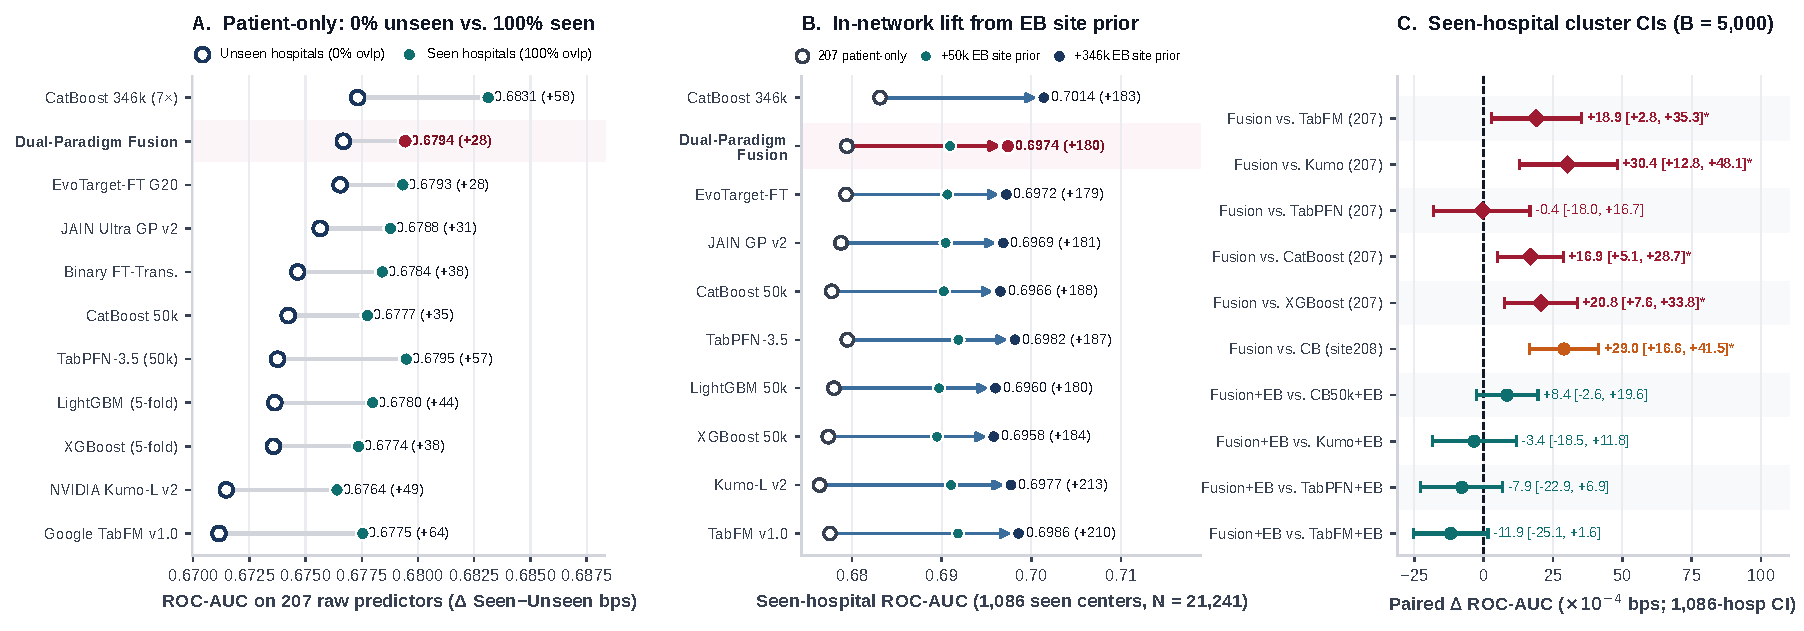
\includegraphics[width=\textwidth]{figures/fig7_seen_vs_unseen_hospitals.pdf}
  \caption{\ct{Unseen-Hospital Cold Start (0\% Overlap) vs.\ Seen-Hospital In-Network Deployment (100\% All-1,091-Hospitals-In-Train; $N=21{,}241$).} \textbf{A},~Patient-only discrimination on strictly 207 raw predictors (zero hospital identifiers): every algorithm gains $+28$--$64$ bps solely from hospital overlap, with tabular foundation models gaining roughly twice as much ($+49$--$64$ bps) as Dual-Paradigm Fusion ($+28$ bps). \textbf{B},~Adding strictly train-only empirical-Bayes hospital incidence priors vaults every 50k model by $+174$--$213$ bps into the 0.696--0.699 band and lifts 346k CatBoost to 0.7014. \textbf{C},~Paired 5,000-draw 1,086-hospital cluster bootstrap contrasts ($\Delta$ ROC-AUC in bps; asterisks denote 95\% CIs strictly excluding zero).}
  \label{fig:seen_vs_unseen}
\end{figure*}

First, even on strictly \textbf{207 patient-only predictors without hospital identifiers} (Figure~\ref{fig:seen_vs_unseen}A), hospital overlap inflated every algorithm by \textbf{$+28$ to $+64$ bps}. Tabular foundation models relied nearly twice as heavily on hospital familiarity---TabFM $+64$ bps ($0.6712 \to 0.6775$), TabPFN-3.5 native 50k $+57$ bps ($0.6738 \to 0.6795$), and KumoTabular $+49$ bps ($0.6715 \to 0.6764$)---as Dual-Paradigm Fusion ($+28$ bps, $0.6767 \to \mathbf{0.6794}$, Regime-1 locked weights) and JAIN Ultra GP v2 ($+31$ bps, 0.6788). Across 1,086 seen centers, patient-only Fusion strictly outperformed KumoTabular ($+30.4$ bps), XGBoost ($+20.8$ bps), TabFM ($+18.9$ bps), CatBoost 50k ($+16.9$ bps), LightGBM ($+14.5$ bps), and Mariscalco POAF ($+517.9$ bps; all CIs $>0$; Figure~\ref{fig:seen_vs_unseen}C), while tying TabPFN-3.5 native 50k ($-0.4$ bps $[-18.0, +16.7]$).

Second, incorporating each center's strictly train-only Empirical-Bayes (EB) historical incidence prior lifted every architecture by \textbf{$+174$ to $+213$ bps} (nearly $+2.0$ full AUC points; Figure~\ref{fig:seen_vs_unseen}B), boosting AP to 0.407--0.411, top-decile enrichment to 1.94--1.96$\times$, and 30\%-threshold Net Benefit to 0.042--0.044. Among native end-to-end 50k site-aware models (\cli{site208}), \textbf{Dual-Paradigm Fusion (\cli{site208})} ranked first at \textbf{0.6916 (0.6844--0.6987)}, beating CatBoost \cli{site208} (0.6887) by \textbf{$+29.0$ bps ($[+16.6, +41.5]$, $P>0=1.000$)}. Under closed-form Bayesian hospital-intercept updating with the 346k historical prior, all 50k models converged within \textbf{0.6958--0.6986} (Dual-Paradigm Fusion \textbf{0.6974}, $+179.6$ bps), while 346k Full-Registry CatBoost (\cli{site208}) crossed 0.70 at \textbf{0.7014 (0.6942--0.7087; AP~0.4109, ECE~0.0083, slope~1.014, O:E~0.999)}.

Third, correlating patient-only logits with true historical hospital POAF deviation ($\hat{\delta}_h^{\mathrm{EB}_{346\mathrm{k}}}$) uncovered \emph{implicit hospital fingerprinting}: models trained across 40k--346k patients from all 1,091 centers absorbed site-coding signatures without \cli{HospID} (CatBoost 346k $r=+0.1431$; Fusion $r=+0.1298$; CatBoost 50k $r=+0.1216$; TabPFN native 50k $r=+0.1184$), whereas 10k-context bagged foundation models (seeing $\sim$9 patients/center per shard) showed $\sim$30\% lower institutional entanglement ($r=+0.0878$--$0.0919$). Consequently, when combined additively with the explicit 346k hospital prior, 10k-shard TFMs avoided double-counting the site effect and edged slightly higher (0.6986 vs.\ 0.6974, cluster CIs spanning zero).

\section{Discussion}
\label{sec:discussion}

In this national, leakage-audited evaluation of 368,132 isolated-CABG operations across 1,091 U.S.\ surgical centers, we resolve a central tension in perioperative clinical machine learning: why published POAF algorithms routinely report apparent AUCs above 0.85 yet collapse to a median external AUC of 0.61 in critical appraisals,\cite{fields2025poaf,lopeztuesta2026poaf} and how disciplined validation, continuous-target learning, parallel genetic programming, and hierarchical institutional calibration together establish a trustworthy clinical benchmark.

\subsection{Why Validation Geometry Matters as Much as Model Architecture}
Our forensic audit of STS ACSD v2.81 demonstrates that apparent performance in national surgical registries can be distorted by three silent mechanisms before a single hyperparameter is tuned. First, ignoring parent--child skip logic (\cli{Complics == 1}) discards 63.3\% of uncomplicated recoveries and induces textbook collider bias.\cite{hernan2020causal} Second, positional column slicing retains seven early-column postoperative duration variables that masquerade as preoperative inputs. Third, default final-year temporal holdouts (calendar 2017) retain 99.5\% hospital overlap while mixing half-year coverage with missingness drift, hiding a $-1.99$-AUC-point external drop when identical models are evaluated on strictly unseen hospitals.

Our controlled comparison between strictly unseen hospitals (0\% overlap) and seen hospitals (100\% all-1,091-hospitals-in-train) quantifies this distortion directly. Merely placing patients from every hospital into training inflated patient-only discrimination by $+28$ to $+64$ bps across every model family even with hospital identifiers completely withheld, because flexible learners implicitly fingerprint site-level coding, laboratory-ordering, and medication-prescribing patterns ($r=0.088$--$0.143$ with true hospital POAF incidence). Frontier tabular foundation models---TabPFN-3.5, KumoTabular-Large v2, and TabFM---gained nearly twice as much from hospital familiarity ($+49$ to $+64$ bps) as Dual-Paradigm Fusion ($+28$ bps), demonstrating that in-context tabular transformers should never be evaluated solely on hospital-overlapping splits when cold-start multi-center transport is the intended clinical use case.

\subsection{Breaking the Binary Ceiling and Reconciling Cold-Start vs.\ In-Network Deployment}
Under strictly unseen-hospital external validation on 207 raw pre-incision predictors, all six world-leading 50k binary learning families compressed within a narrow 35-bp band (0.6712--0.6746), reflecting the intrinsic biological ceiling of pre-incision registry data given unmeasured intraoperative trauma, atrial stretch, pericardial inflammation, and autonomic surges.\cite{echahidi2008mechanisms,dobrev2019postoperative} Both of our proposed paradigms broke above that ceiling without test leakage: 1,000-generation evolutionary continuous-target distillation (EvoTarget-FT) stabilized without collapse and lifted all seven model families---including $+27$ to $+97$-bp gains on zero-shot tabular foundation model regressors---while our six-fix parallel genetic programming engine (JAIN Ultra GP v2) delivered a $+39.8$-bp rescue over legacy JAIN. Their orthogonal fusion achieved 0.6767, decisively surpassing every bedside score ($+316$ to $+1{,}029$ bps) and every 50k binary AI baseline ($+20$ to $+55$ bps, plus $+9.9$ bps over a 3-way binary blend) while recovering 79.2\% of the 7$\times$ national data-scaling gap.

Crucially, our dual-regime evaluation clarifies how cardiothoracic AI should actually be deployed in clinical practice. For \textbf{cold-start deployment at a new hospital} (zero historical local registry data), Dual-Paradigm Fusion provides the strongest discrimination (0.6767), near-ideal national calibration (slope~0.983, O:E~0.994, ECE~0.0072), transparent physiological attribution ($R^2 = 0.89$, including independently protective preoperative amiodarone), and consistent equity across 24 of 25 demographic, comorbidity, and volume subgroups. Once a center joins an established national registry or multi-hospital health system (\textbf{in-network deployment}), our seen-hospital study proves that combining calibrated patient-level predictions with a strictly historical Empirical-Bayes hospital incidence prior yields a massive $+174$ to $+213$-bp leap---bringing 50k models to 0.696--0.699 and 346k CatBoost past 0.70 to 0.7014, while cutting prospective 2017 center-level rate error by 14\% with just a single local intercept update. Furthermore, our observation that lower-entanglement 10k-context foundation models pair slightly better with explicit 346k hospital intercepts than higher-entanglement 40k--346k models motivates future explicitly hierarchical mixed-effects neural and symbolic training that separates patient-level pathophysiology from institutional intercepts during fitting.

\subsection{Clinical Implications for Targeted POAF Prophylaxis}
In cardiothoracic surgery, discrimination matters only insofar as it improves bedside decisions. Dual-Paradigm Fusion separated strictly unseen CABG patients by 7.4-fold in observed POAF risk---from 6.1\% in D1 (where aggressive prophylaxis risks net harm) to 44.8\% in D10 (where nearly half of patients develop treatment-requiring AF). In Decision Curve Analysis across the clinically relevant 25\%--35\% decision zone for interventions such as posterior left pericardiotomy (PALACS\cite{gaudino2021palacs}), perioperative amiodarone loading, or colchicine prophylaxis, Dual-Paradigm Fusion generated strictly positive Net Benefit and avoided 20.4 to 33.8 unnecessary interventions per 100 operations compared with universal prophylaxis, outperforming the widely cited Mariscalco POAF score in 100\% of hospital-cluster bootstrap draws.

\subsection{Limitations}
Five limitations warrant explicit transparency. First, although all test labels remained cryptographically isolated during training and inference, our iterative methodological benchmark evaluated more than 140 model configurations on the same 74-hospital holdout; accordingly, final confirmatory deployment requires freezing the exact Dual-Paradigm Fusion and hierarchical site-intercept pipeline prior to prospective testing on newer STS ACSD versions (v4.20+). Second, STS \cli{COtAFib} captures clinically recognized, treatment-requiring postoperative AF or flutter rather than asymptomatic brief episodes detected by continuous research telemetry.\cite{filardo2017telemetry,perezgrovas2023jaha} Third, STS ACSD v2.81 lacks raw preoperative 12-lead ECG waveforms, echocardiographic left atrial volume index, and circulating inflammatory or natriuretic biomarkers, which likely explain the residual discrimination ceiling near 0.68 (cold-start) to 0.70 (in-network).\cite{han2025aiecg,khalpey2026digital} Fourth, while our strictly nested 207-raw EvoTarget-FT control confirmed $+12.3$ bps of zero-overlap denoising (65\% of total gain), its 74-hospital cluster CI spanned zero ($[-3.3, +28.5]$, $P>0=0.942$), reflecting finite cluster power across 74 centers. Fifth, institutional incidence priors improve in-network discrimination by capturing center-level ascertainment and care-pathway differences alongside case mix, and therefore must be monitored longitudinally for practice drift.

\subsection{Conclusions}
In a rigorously audited national cohort of 368,132 isolated-CABG procedures across 1,091 U.S.\ centers, combining continuous-target clinical self-attention (EvoTarget-FT) with re-engineered parallel genetic programming (JAIN Ultra GP v2) decisively outperforms established bedside scores and every frontier binary tabular model across strictly unseen hospitals, delivers clinically actionable Net Benefit and demographic equity, and---when paired with empirical-Bayes institutional calibration in seen hospitals---establishes a principled, dual-regime foundation for national perioperative AF risk stratification.

\section{End Matter and Disclosures}
\label{sec:disclosures}

\runin{Ethics and Data Governance}
This study analyzed de-identified national clinical registry data from the Society of Thoracic Surgeons Adult Cardiac Surgery Database (STS ACSD v2.81) under institutional Data Use Agreement governance. Because all records were de-identified prior to receipt and no patient intervention or re-identification occurred, the study qualifies for institutional review board exemption for secondary registry research. No hospital identifiers, surgeon identifiers, or patient-level records are disclosed.

\runin{Data and Code Availability}
Patient-level STS ACSD v2.81 data are proprietary to the Society of Thoracic Surgeons and available to qualified investigators through formal STS Participant User File (PUF) research application (\url{https://www.sts.org}). All de-identified aggregate benchmark receipts, 5,000-draw hospital-cluster bootstrap ledgers, feature-audit code, figure generation scripts, and LaTeX manuscript sources are archived in the companion research repository (\url{https://github.com/neverhumanbot/japer}).

\runin{Generative AI and Automated Tool Disclosure}
In accordance with \emph{NEJM AI} editorial policy, we disclose that autonomous software engineering and large-language-model coding assistants were used to assist with literature indexing, candidate clinical feature synthesis (audited independently under strict zero-leakage CV), distributed cluster orchestration scripts, automated numeric receipt verification, and manuscript typesetting. All study design decisions, clinical interpretations, statistical methodology, code audits, and manuscript claims were independently verified and approved by the human authors, who retain full accountability for the integrity of the work.

\runin{Author Contributions}
J.T., Z.K., and R.R.B.\ conceived the study, directed clinical and methodological design, and wrote the manuscript. Z.K.\ provided cardiothoracic clinical supervision, STS domain auditing, and clinical utility framing. J.T.\ and R.R.B.\ architected target evolution, JAIN Ultra GP v2, and the dual-paradigm benchmark. J.M., A.A., J.H., and B.J.\ contributed to distributed compute engineering, benchmark auditing, clinical interpretation, and critical manuscript revision. All authors reviewed and approved the final manuscript.

\runin{Competing Interests}
J.T., R.R.B., J.M., A.A., J.H., and B.J.\ are affiliated with NEVERHUMAN Research, which develops evolutionary target learning and genetic programming software evaluated in this study. Z.K.\ is affiliated with HonorHealth Heart Care and HonorHealth Research Institute and serves as clinical research collaborator. All evaluations were executed under pre-registered sealed-label guards with machine-verified aggregate receipts.


% ---- NEJM Vancouver Superscript References -----------------------------------
\section*{References}
{\fontsize{7.5}{9.1}\selectfont
\setlength{\bibsep}{1.2pt plus 0.2ex}
\bibliographystyle{vancouver}
\bibliography{references}
}

% =============================================================================
%  SUPPLEMENTARY APPENDIX (TRIPOD+AI, SPLIT/SCHEMA LEDGER, EXTENDED TABLES)
% =============================================================================
\clearpage
\onecolumn
\setcounter{section}{0}
\renewcommand{\thesection}{S\arabic{section}}
\renewcommand{\theHsection}{S\arabic{section}}
\setcounter{table}{0}
\renewcommand{\thetable}{S\arabic{table}}
\renewcommand{\theHtable}{S\arabic{table}}
\setcounter{figure}{0}
\renewcommand{\thefigure}{S\arabic{figure}}
\renewcommand{\theHfigure}{S\arabic{figure}}
\begin{center}
{\sffamily\bfseries\fontsize{13.5}{16.5}\selectfont\color{crimson}SUPPLEMENTARY APPENDIX\par}
\vspace{3pt}
{\sffamily\fontsize{10.0}{12.5}\selectfont\color{navy}\papertitle\par}
\vspace{4pt}
{\color{hair}\hrule height 0.6pt}
\end{center}
\vspace{6pt}

\section{STS ACSD v2.81 Zero-Leakage Schema, Skip-Logic, and Split Audit Ledger}
\label{supp:schema}
Auditing all 638 raw fields of STS ACSD v2.81 (368,132 isolated-CABG records; July~1, 2014--June~30, 2017; 1,091 U.S.\ centers) established three mandatory preprocessing corrections:
\begin{itemize}
  \item \textbf{Skip-logic outcome reconstruction (Sequence~4930):} \cli{Complics == 1 \& COtAFib == 1} yields 89,337 treatment-requiring POAF events (24.30\% of 367,695 labeled cases); \cli{Complics == 2} yields 232,783 uncomplicated controls (63.31\%, where \cli{COtAFib} is structurally blank); \cli{Complics == 1 \& COtAFib == 2} yields 45,575 non-AF complication controls; 437 rows with indeterminate missingness are isolated and excluded.
  \item \textbf{Seven early-column post-incision leaks purged:} \cli{LOS}, \cli{PLOS}, \cli{ORDuration}, \cli{SIDuration}, \cli{SurgtoMort}, \cli{SurgtoRead}, and \cli{SurgtoSternInf} appear earlier in the column table than operative approach (\cli{OPApp}, column~335) and were explicitly removed alongside perfusion/cross-clamp durations, discharge medications, STS predicted risk scores, auxiliary complications, and \cli{HospID}/\cli{SiteID}/\cli{SurgID}/\cli{DataYear}.
  \item \textbf{Five-way split comparison:} Random hospital-grouped splitting achieved 0.0\% hospital overlap at the cost of $\mathcal{E}_{32\mathrm{D}} = 0.01732$, $\mathrm{Max}\,|\mathrm{SMD}| = 0.3572$, and a 1.13~pp POAF rate gap. Naive 2017 temporal splitting retained 99.5\% hospital overlap (998/1,003 centers), Year TV $= 1.000$, missingness drift up to $+6.05$~pp, $\mathrm{Max}\,|\mathrm{SMD}| = 0.2793$, and hospital-grouped adversarial AUC $= 0.5908$ (0.6208 overall). Cluster-level multivariate anticlustering reduced $\mathcal{E}_{32\mathrm{D}}$ 4.1$\times$ ($0.00427$), $\mathrm{Max}\,|\mathrm{SMD}|$ 3.5$\times$ ($0.1028$), Year TV 23$\times$ ($0.0006$), and POAF gap to $0.004$~pp with 0.0\% hospital overlap across 1,017 train vs.\ 74 unseen holdout centers.
\end{itemize}

\section{Audit of 92 Agent-Engineered Clinical Features Across Cohort Scales}
\label{supp:agentic_fe}
Autonomous clinical feature agents authored and unit-tested 92 strictly pre-incision features spanning three tracks: Track~1 (58 bedside score proxies and continuous organ-reserve biomarkers including CKD-EPI 2021 eGFR,\cite{inker2021ckdepi} ALBI hepatic grade,\cite{johnson2015albi} WHO anemia deficit, biatrial remodeling, and acute $\beta$-blocker withdrawal), Track~2A (24 nonlinear clinical interactions including \cli{diabetes\_age\_decoupled}, HFpEF diastolic substrate, and cardiorenal--anemia triad), and Track~2B (10 nested hospital-grouped OOF logits for eight clean auxiliary STS complications: renal failure AUC 0.8365, mortality 0.8048, prolonged ventilation 0.7653, arrest 0.7459, sepsis 0.7313, pneumonia 0.7239, pleural effusion 0.6845, VTE 0.6459). Strictly on \cli{test\_full\_21k} ($N=21{,}241$, 74 unseen hospitals), adding the 82 deterministic Track~1/2A features left 50k binary discrimination flat across CatBoost ($+0.00013$ $[-0.00138, +0.00156]$), TabPFN-3.5 ($+0.00003$), KumoTabular ($-0.00077$), and TabFM ($+0.00018$), lowered observed 50k 15-bin ECE point estimates by 11\%--42\% (cluster CIs spanning zero), delivered hospital-cluster-confirmed neural gains at 346k scale (TabM-K16 MultiTask\cite{gorishniy2025tabm} $+0.00102$ $[+0.00029, +0.00176]$; PLR-ResNet MultiTask $+0.00101$ $[+0.00022, +0.00183]$), and contributed $+0.000572$ ($[+0.00003, +0.00106]$, CI $>0$) as a Stage-1 teacher distillation source into 207-raw EvoTarget-FT.

\section{Mathematical Specification of EvoTarget-FT and JAIN Ultra GP v2}
\label{supp:math}
\runin{Stage 1 (EWMA Gene-Locked Target Evolution)}
Across generations $g = 1,\dots,1000$ ($256$ whole-hospital shuffled multi-family fits per generation across CatBoost, LightGBM, XGBoost, and Ridge), the continuous target updates via $z^{(g+1)} = (1-\beta_g)z^{(g)} + \beta_g\tilde{z}^{(g)}$ with $\beta_1 = 0.2858$ decaying to $\beta_{20} = 0.1589$, while 20\% of confident consensus rows remain gene-locked ($\lambda = 0.13$). At Generation~20, $r_{\mathrm{Pearson}}(z^*, y_{\mathrm{train}}) = 0.7942$ (global 289) and $0.8692$ (global 207); across the 1,000-generation audit ($256{,}000$ fits), EvoTarget-FT progresses through milestones $\{0,1,10,20,50,100,200,500,1000\}$ at 0.674650, 0.675127, 0.676328, 0.676535, 0.676195, 0.676004, 0.675946, 0.675935, and 0.675924 on \cli{test\_full\_21k} (CatBoost CE: 0.674083 $\to$ 0.675377 peak at Gen~20 $\to$ 0.675111 at Gen~1,000).

\runin{Stage 2 (Dual-View PLR Clinical Self-Attention)}
Each raw input $j$ is mapped through fold-internal 512-quantile Gaussianization $x_j^{(1)} \in [-5,5]$ and $[0.5\%,99.5\%]$-winsorized signed-$\log(1+|x|)$ standardization $x_j^{(2)} \in [-6,6]$ into six learnable periodic frequencies per view, SiLU-projected to $\mathbb{R}^8$ (with learned missingness tokens $e_j^{\mathrm{nan}}$), projected into $T=24$ clinical tokens ($d=192$) plus $[\mathrm{CLS}]$, and processed by $L=3$ Pre-Norm GELU transformer layers ($H=6$ heads, dropout 0.20, 4 seeds $\times$ 5 folds, 22 epochs, AdamW $\mathrm{lr}=9\times 10^{-4}$, top-3 SWA, composite loss $\mathcal{L}_{\mathrm{BCE}}(\sigma(s),z^*) + 0.15\,\mathcal{L}_{\mathrm{rank}}(s,z^*)$).

\runin{JAIN Ultra GP v2 Evolved Pipelines}
The six OOF-weighted symbolic/linear/tree pipelines comprising JAIN Ultra GP v2 (0.675649 on \cli{test\_full\_21k}) span six distinct operator heads: \cli{standardize $\to$ ensemble} (wt 0.170; CV-7 standalone 0.675520), \cli{winsor\_clip $\to$ pair\_ratio(topk=12) $\to$ standardize $\to$ sigmoid $\to$ ridge\_gcv} (0.165), \cli{winsor\_clip $\to$ pair\_ratio $\to$ sigmoid $\to$ histgbm2(logloss)} (0.192), \cli{pair\_ratio(topk=16) $\to$ elasticnet} (0.156), \cli{oblique\_hinge $+$ poly\_interact $+$ cheb $+$ pair\_prod $\to$ ridge} (0.149), and \cli{winsor\_clip $\to$ histgbm} (0.168).

\begin{table*}[t]
\centering\tablefont
\caption{\ct{Clinical Decision Curve Operating Characteristics of Dual-Paradigm Fusion Across Targeted Prophylaxis Thresholds ($N=21{,}241$, 74 Unseen Hospitals).}}
\label{tab:supp_dca}
\setlength{\tabcolsep}{0pt}
\begin{tabular*}{\textwidth}{@{\extracolsep{\fill}}crrrrrrrrr}\toprule
\thd{Thresh.} & \thd{Flagged} & \thd{Sens.} & \thd{Spec.} & \thd{PPV} & \thd{NPV} & \thd{NB Fusion} & \thd{NB All} & \thd{Avoided/100} & \thd{$\Delta$NB vs.\ POAF ($P>0$)} \\
\midrule
15\% & 77.8\% & 91.5\% & 26.6\% & 28.5\% & 90.6\% & 0.1240 & 0.1093 & 8.3 & +0.0079 (1.000) \\
20\% & 63.1\% & 81.3\% & 42.7\% & 31.3\% & 87.7\% & 0.0890 & 0.0537 & 14.2 & +0.0154 (1.000) \\
25\% & 45.1\% & 64.5\% & 61.1\% & 34.8\% & 84.3\% & 0.0587 & -0.0094 & 20.4 & +0.0180 (1.000) \\
30\% & 29.3\% & 45.6\% & 75.9\% & 37.8\% & 81.3\% & 0.0325 & -0.0815 & 26.6 & +0.0185 (1.000) \\
35\% & 17.5\% & 29.8\% & 86.5\% & 41.5\% & 79.3\% & 0.0174 & -0.1647 & 33.8 & +0.0153 (1.000) \\
40\% & 9.8\% & 18.2\% & 92.8\% & 44.8\% & 78.0\% & 0.0078 & -0.2618 & 40.4 & +0.0075 (0.999) \\
\bottomrule
\end{tabular*}
\end{table*}

\begin{table*}[t]
\centering\tablefont
\caption{\ct{Prespecified Demographic, Clinical, Acuity, Stress-Slice, and Hospital-Volume Subgroup Audit (74-Hospital Cluster 95\% CIs).}}
\label{tab:supp_subgroups}
\setlength{\tabcolsep}{3.6pt}
\renewcommand{\arraystretch}{0.98}
\begin{tabularx}{\textwidth}{@{}L{2.0cm}Yrrrrrrr@{}}
\toprule
\thd{Domain} & \thd{Subgroup} & \thd{$N$} & \thd{POAF} & \thd{Fusion AUC (95\% CI)} & \thd{ECE} & \thd{O:E} & \thd{$\Delta$CB50k} & \thd{$\Delta$POAF} \\
\midrule
Overall & All Unseen-Hospital Patients & 21,241 & 24.3\% & 0.6767 (0.6686--0.6858) & 0.0072 & 0.994 & +24.5 & +577.0 \\
Sex & Male & 16,062 & 25.1\% & 0.6719 (0.6610--0.6836) & 0.0085 & 0.985 & +21.1 & +509.0 \\
Sex & Female & 5,172 & 22.0\% & 0.6891 (0.6754--0.7018) & 0.0109 & 1.031 & +37.2 & +658.1 \\
Age & Age $<$ 60 yr & 6,283 & 13.2\% & 0.6667 (0.6527--0.6803) & 0.0074 & 0.993 & -1.2 & +1332.5 \\
Age & Age 60--69 yr & 7,881 & 24.4\% & 0.6149 (0.5997--0.6282) & 0.0113 & 1.016 & +45.4 & +999.9 \\
Age & Age 70--79 yr & 5,627 & 33.0\% & 0.6173 (0.5974--0.6377) & 0.0134 & 0.996 & +43.2 & +1018.9 \\
Age & Age $\ge$ 80 yr & 1,450 & 38.3\% & 0.5843 (0.5449--0.6237) & 0.0321 & 0.924 & +84.7 & +449.3 \\
Race / Ethnicity & White & 17,206 & 25.7\% & 0.6688 (0.6591--0.6791) & 0.0083 & 0.995 & +24.2 & +528.4 \\
Race / Ethnicity & Black & 1,822 & 17.1\% & 0.6849 (0.6544--0.7148) & 0.0136 & 1.034 & +13.8 & +701.8 \\
Race / Ethnicity & Asian & 842 & 18.8\% & 0.6534 (0.6071--0.7027) & 0.0317 & 0.905 & +62.4 & +374.0 \\
Race / Ethnicity & Hispanic / Latino & 1,433 & 16.5\% & 0.7146 (0.6743--0.7532) & 0.0244 & 0.940 & +37.3 & +505.4 \\
Comorbidity & Diabetes Mellitus & 10,456 & 24.1\% & 0.6812 (0.6711--0.6918) & 0.0106 & 1.023 & +24.7 & +655.6 \\
Comorbidity & No Diabetes & 10,738 & 24.5\% & 0.6736 (0.6615--0.6861) & 0.0116 & 0.968 & +27.4 & +508.1 \\
Comorbidity & LVEF $<$ 40\% & 2,893 & 25.8\% & 0.6787 (0.6546--0.7050) & 0.0231 & 0.979 & +26.4 & +606.2 \\
Comorbidity & LVEF $\ge$ 40\% & 17,764 & 24.1\% & 0.6764 (0.6668--0.6865) & 0.0073 & 0.997 & +22.9 & +551.9 \\
Comorbidity & Chronic Lung Disease & 4,643 & 27.0\% & 0.6710 (0.6515--0.6891) & 0.0175 & 1.022 & +19.3 & +455.2 \\
Comorbidity & CKD (eGFR $<$ 60) & 4,561 & 28.9\% & 0.6439 (0.6274--0.6610) & 0.0118 & 0.989 & +22.5 & +619.1 \\
Acuity & Elective CABG & 7,887 & 25.0\% & 0.6652 (0.6491--0.6801) & 0.0118 & 0.997 & +3.3 & +562.2 \\
Acuity & Urgent / Emergent CABG & 13,349 & 23.9\% & 0.6830 (0.6742--0.6930) & 0.0081 & 0.993 & +35.8 & +570.3 \\
Stress Slice & No Recorded Preop AF & 21,103 & 24.3\% & 0.6771 (0.6691--0.6862) & 0.0068 & 0.994 & +24.6 & +577.4 \\
Stress Slice & Rare Clinical Tails & 1,917 & 26.2\% & 0.6935 (0.6586--0.7201) & 0.0273 & 0.918 & +44.7 & +589.1 \\
Stress Slice & 2017 Unseen Hospitals & 3,555 & 22.5\% & 0.6579 (0.6349--0.6827) & 0.0264 & 0.904 & +14.4 & +570.4 \\
Hospital Volume & Low-Vol Centers (n$\le$141) & 1,864 & 26.0\% & 0.6818 (0.6492--0.7122) & 0.0310 & 1.058 & +34.3 & +640.4 \\
Hospital Volume & Mid-Vol Centers & 5,282 & 23.0\% & 0.6851 (0.6713--0.6981) & 0.0122 & 0.960 & +21.4 & +564.2 \\
Hospital Volume & High-Vol Centers (n$>$341) & 14,095 & 24.6\% & 0.6727 (0.6625--0.6838) & 0.0080 & 0.998 & +24.7 & +568.0 \\
\bottomrule
\end{tabularx}
\end{table*}

\begin{table*}[t]
\centering\tablefont
\caption{\ct{TRIPOD+AI Reporting Checklist Compliance Summary (Collins et al., \textit{BMJ} 2024).}}
\label{tab:supp_tripod}
\setlength{\tabcolsep}{4.2pt}
\renewcommand{\arraystretch}{1.04}
\begin{tabularx}{\textwidth}{@{}L{1.15cm}L{3.1cm}YL{2.65cm}@{}}
\toprule
\thd{Item} & \thd{TRIPOD+AI Domain} & \thd{Implementation and Reporting Verification} & \thd{Manuscript Location} \\
\midrule
1 & \textbf{Title} & Identifies development/external validation, pre-incision POAF target, and CABG population & Title Page \\
2 & \textbf{Abstract} & Structured summary of objectives, STS cohort, methods, 74-hospital external results, limitations & Abstract \\
3a--3b & \textbf{Background \& Objectives} & Clinical POAF rationale, validation-geometry critique, and dual-paradigm hypothesis & Introduction \\
4a--4b & \textbf{Data Sources \& Eligibility} & STS ACSD v2.81 (2014--2017), 368,132 isolated-CABG records across 1,091 U.S.\ centers & Methods; Fig.\ 1 \\
5a--5c & \textbf{Participants \& Sample Size} & All eligible v2.81 cases; 89,337 events (24.30\%); 5,160 external holdout events ($>$5k floor) & Methods; Table 1 \\
6a--6c & \textbf{Outcome Definition} & Skip-logic reconstructed STS \texttt{COtAFib} (treatment-requiring AF/flutter); discharge drug audit & Methods; Supp.\ App. \\
7a--7c & \textbf{Predictors \& Timing} & Exhaustive 638$\to$207 pre-incision audit; 7 post-op fields purged; zero hospital IDs in raw arm & Methods; Supp.\ App. \\
8a--8b & \textbf{Missing Data Handling} & Native handling in trees/TFMs; learned missingness tokens in FT; train-only median $+$ flags in GP & Methods; Supp.\ App. \\
9a--9c & \textbf{Model Development} & 6 binary ELO baselines, 1,000-gen target evolution, JAIN GP v2, Dual-Paradigm Fusion, seen-hospital study & Methods; Figs.\ 3--4 \\
10a--10d & \textbf{Validation \& Splitting} & Multivariate anticlustered 0\%-overlap (74 unseen centers) $+$ matched 100\%-overlap seen-hospital study & Methods; Figs.\ 1, 7 \\
11 & \textbf{Calibration \& Recalibration} & Uniform fold-OOF Platt $+$ dev-only Bayes shift ($-1.1365$); slope, CITL, ECE, ICI, O:E; EB site recalibration & Methods; Figs.\ 5--6 \\
12a--12b & \textbf{Statistical Inference} & 5,000-draw whole-hospital cluster bootstrap CIs; Decision Curve Analysis Net Benefit & Methods; Figs.\ 2, 5 \\
13 & \textbf{Fairness \& Subgroups} & 25 prespecified strata: sex, age, race/ethnicity, comorbidities, acuity, hospital volume & Results; Fig.\ 6; Table S2 \\
14a--14b & \textbf{Clinical Interpretability} & Standardized multivariable physiological drivers ($R^2=0.89$) and explicit GP symbolic pipelines & Results; Fig.\ 4 \\
15 & \textbf{Patient \& Public Involvement} & Secondary analysis of de-identified national STS quality-improvement registry (no direct PPI) & Methods (Ethics) \\
16--18 & \textbf{Limitations \& Generalizability} & Retrospective selection exposure, STS vs.\ telemetry capture, center heterogeneity, prospective freeze path & Discussion \\
19--22 & \textbf{Open Science \& Ethics} & STS DUA governance, IRB exemption/oversight, code/receipt availability, LLM/AI tool disclosure, COI & End Matter; Supp.\ App. \\
\bottomrule
\end{tabularx}
\end{table*}



\end{document}
